% polymake for william
% Tue May  2 09:09:50 2017
% skel

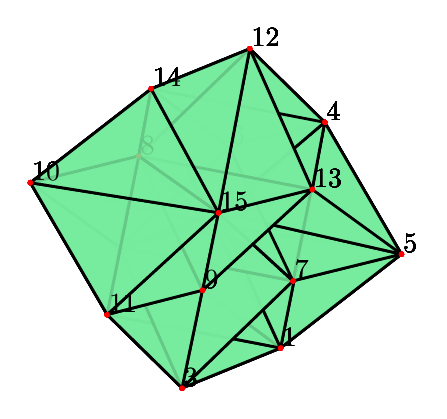
\begin{tikzpicture}[x  = {(0.9cm,-0.076cm)},
                    y  = {(-0.06cm,0.95cm)},
                    z  = {(-0.44cm,-0.29cm)},
                    scale = 1,
                    color = {lightgray}]


  % POINTS STYLE
  \definecolor{pointcolor_GRAPHofskel}{rgb}{ 0,0,0 }
  \tikzstyle{pointstyle_GRAPHofskel} = [fill=pointcolor_GRAPHofskel]

  % DEF POINTS
  \coordinate (v0_GRAPHofskel) at (-0.0375869, -0.0774062, 0.00785973);
  \coordinate (v1_GRAPHofskel) at (0.606698, -1.79913, -0.380721);
  \coordinate (v2_GRAPHofskel) at (-0.428789, 0.152126, 1.88221);
  \coordinate (v3_GRAPHofskel) at (0.190013, -1.76179, 1.60645);
  \coordinate (v4_GRAPHofskel) at (1.40016, 1.26082, -0.447153);
  \coordinate (v5_GRAPHofskel) at (2.14607, -0.575955, -0.885162);
  \coordinate (v6_GRAPHofskel) at (1.03886, 1.51133, 1.53535);
  \coordinate (v7_GRAPHofskel) at (1.57745, -0.38631, 1.0546);
  \coordinate (v8_GRAPHofskel) at (-1.57748, 0.38629, -1.05456);
  \coordinate (v9_GRAPHofskel) at (-1.03862, -1.5112, -1.53563);
  \coordinate (v10_GRAPHofskel) at (-2.14601, 0.575815, 0.885389);
  \coordinate (v11_GRAPHofskel) at (-1.40017, -1.26083, 0.447088);
  \coordinate (v12_GRAPHofskel) at (-0.190304, 1.76181, -1.6064);
  \coordinate (v13_GRAPHofskel) at (0.428841, -0.152086, -1.8822);
  \coordinate (v14_GRAPHofskel) at (-0.606711, 1.79912, 0.380742);
  \coordinate (v15_GRAPHofskel) at (0.0375869, 0.0774062, -0.00785974);



  % EDGE STYLE
  \definecolor{linecolor_GRAPHofskel}{rgb}{ 0 0 0 }

  \tikzstyle{linestyle_GRAPHofskel} = [color=linecolor_GRAPHofskel, thick]


  % EDGES
  \draw[linestyle_GRAPHofskel] (v1_GRAPHofskel) -- (v0_GRAPHofskel);
  \draw[linestyle_GRAPHofskel] (v2_GRAPHofskel) -- (v0_GRAPHofskel);
  \draw[linestyle_GRAPHofskel] (v3_GRAPHofskel) -- (v0_GRAPHofskel);
  \draw[linestyle_GRAPHofskel] (v3_GRAPHofskel) -- (v1_GRAPHofskel);
  \draw[linestyle_GRAPHofskel] (v3_GRAPHofskel) -- (v2_GRAPHofskel);
  \draw[linestyle_GRAPHofskel] (v4_GRAPHofskel) -- (v0_GRAPHofskel);
  \draw[linestyle_GRAPHofskel] (v5_GRAPHofskel) -- (v0_GRAPHofskel);
  \draw[linestyle_GRAPHofskel] (v5_GRAPHofskel) -- (v1_GRAPHofskel);
  \draw[linestyle_GRAPHofskel] (v5_GRAPHofskel) -- (v4_GRAPHofskel);
  \draw[linestyle_GRAPHofskel] (v6_GRAPHofskel) -- (v0_GRAPHofskel);
  \draw[linestyle_GRAPHofskel] (v6_GRAPHofskel) -- (v2_GRAPHofskel);
  \draw[linestyle_GRAPHofskel] (v6_GRAPHofskel) -- (v4_GRAPHofskel);
  \draw[linestyle_GRAPHofskel] (v7_GRAPHofskel) -- (v0_GRAPHofskel);
  \draw[linestyle_GRAPHofskel] (v7_GRAPHofskel) -- (v1_GRAPHofskel);
  \draw[linestyle_GRAPHofskel] (v7_GRAPHofskel) -- (v2_GRAPHofskel);
  \draw[linestyle_GRAPHofskel] (v7_GRAPHofskel) -- (v3_GRAPHofskel);
  \draw[linestyle_GRAPHofskel] (v7_GRAPHofskel) -- (v4_GRAPHofskel);
  \draw[linestyle_GRAPHofskel] (v7_GRAPHofskel) -- (v5_GRAPHofskel);
  \draw[linestyle_GRAPHofskel] (v7_GRAPHofskel) -- (v6_GRAPHofskel);
  \draw[linestyle_GRAPHofskel] (v8_GRAPHofskel) -- (v0_GRAPHofskel);
  \draw[linestyle_GRAPHofskel] (v9_GRAPHofskel) -- (v0_GRAPHofskel);
  \draw[linestyle_GRAPHofskel] (v9_GRAPHofskel) -- (v1_GRAPHofskel);
  \draw[linestyle_GRAPHofskel] (v9_GRAPHofskel) -- (v8_GRAPHofskel);
  \draw[linestyle_GRAPHofskel] (v10_GRAPHofskel) -- (v0_GRAPHofskel);
  \draw[linestyle_GRAPHofskel] (v10_GRAPHofskel) -- (v2_GRAPHofskel);
  \draw[linestyle_GRAPHofskel] (v10_GRAPHofskel) -- (v8_GRAPHofskel);
  \draw[linestyle_GRAPHofskel] (v11_GRAPHofskel) -- (v0_GRAPHofskel);
  \draw[linestyle_GRAPHofskel] (v11_GRAPHofskel) -- (v1_GRAPHofskel);
  \draw[linestyle_GRAPHofskel] (v11_GRAPHofskel) -- (v2_GRAPHofskel);
  \draw[linestyle_GRAPHofskel] (v11_GRAPHofskel) -- (v3_GRAPHofskel);
  \draw[linestyle_GRAPHofskel] (v11_GRAPHofskel) -- (v8_GRAPHofskel);
  \draw[linestyle_GRAPHofskel] (v11_GRAPHofskel) -- (v9_GRAPHofskel);
  \draw[linestyle_GRAPHofskel] (v11_GRAPHofskel) -- (v10_GRAPHofskel);
  \draw[linestyle_GRAPHofskel] (v12_GRAPHofskel) -- (v0_GRAPHofskel);
  \draw[linestyle_GRAPHofskel] (v12_GRAPHofskel) -- (v4_GRAPHofskel);
  \draw[linestyle_GRAPHofskel] (v12_GRAPHofskel) -- (v8_GRAPHofskel);
  \draw[linestyle_GRAPHofskel] (v13_GRAPHofskel) -- (v0_GRAPHofskel);
  \draw[linestyle_GRAPHofskel] (v13_GRAPHofskel) -- (v1_GRAPHofskel);
  \draw[linestyle_GRAPHofskel] (v13_GRAPHofskel) -- (v4_GRAPHofskel);
  \draw[linestyle_GRAPHofskel] (v13_GRAPHofskel) -- (v5_GRAPHofskel);
  \draw[linestyle_GRAPHofskel] (v13_GRAPHofskel) -- (v8_GRAPHofskel);
  \draw[linestyle_GRAPHofskel] (v13_GRAPHofskel) -- (v9_GRAPHofskel);
  \draw[linestyle_GRAPHofskel] (v13_GRAPHofskel) -- (v12_GRAPHofskel);
  \draw[linestyle_GRAPHofskel] (v14_GRAPHofskel) -- (v0_GRAPHofskel);
  \draw[linestyle_GRAPHofskel] (v14_GRAPHofskel) -- (v2_GRAPHofskel);
  \draw[linestyle_GRAPHofskel] (v14_GRAPHofskel) -- (v4_GRAPHofskel);
  \draw[linestyle_GRAPHofskel] (v14_GRAPHofskel) -- (v6_GRAPHofskel);
  \draw[linestyle_GRAPHofskel] (v14_GRAPHofskel) -- (v8_GRAPHofskel);
  \draw[linestyle_GRAPHofskel] (v14_GRAPHofskel) -- (v10_GRAPHofskel);
  \draw[linestyle_GRAPHofskel] (v14_GRAPHofskel) -- (v12_GRAPHofskel);
  \draw[linestyle_GRAPHofskel] (v15_GRAPHofskel) -- (v0_GRAPHofskel);


  %POINTS
  \node at (v0_GRAPHofskel) [inner sep=0.5pt, above right, black,align=left] {0};
  \fill[pointcolor_GRAPHofskel] (v0_GRAPHofskel) circle (1 pt);


  %EDGES
  \draw[linestyle_GRAPHofskel] (v15_GRAPHofskel) -- (v1_GRAPHofskel);


  %POINTS
  \node at (v1_GRAPHofskel) [inner sep=0.5pt, above right, black,align=left] {1};
  \fill[pointcolor_GRAPHofskel] (v1_GRAPHofskel) circle (1 pt);


  %EDGES
  \draw[linestyle_GRAPHofskel] (v15_GRAPHofskel) -- (v2_GRAPHofskel);


  %POINTS
  \node at (v2_GRAPHofskel) [inner sep=0.5pt, above right, black,align=left] {2};
  \fill[pointcolor_GRAPHofskel] (v2_GRAPHofskel) circle (1 pt);


  %EDGES
  \draw[linestyle_GRAPHofskel] (v15_GRAPHofskel) -- (v3_GRAPHofskel);


  %POINTS
  \node at (v3_GRAPHofskel) [inner sep=0.5pt, above right, black,align=left] {3};
  \fill[pointcolor_GRAPHofskel] (v3_GRAPHofskel) circle (1 pt);


  %EDGES
  \draw[linestyle_GRAPHofskel] (v15_GRAPHofskel) -- (v4_GRAPHofskel);


  %POINTS
  \node at (v4_GRAPHofskel) [inner sep=0.5pt, above right, black,align=left] {4};
  \fill[pointcolor_GRAPHofskel] (v4_GRAPHofskel) circle (1 pt);


  %EDGES
  \draw[linestyle_GRAPHofskel] (v15_GRAPHofskel) -- (v5_GRAPHofskel);


  %POINTS
  \node at (v5_GRAPHofskel) [inner sep=0.5pt, above right, black,align=left] {5};
  \fill[pointcolor_GRAPHofskel] (v5_GRAPHofskel) circle (1 pt);


  %EDGES
  \draw[linestyle_GRAPHofskel] (v15_GRAPHofskel) -- (v6_GRAPHofskel);


  %POINTS
  \node at (v6_GRAPHofskel) [inner sep=0.5pt, above right, black,align=left] {6};
  \fill[pointcolor_GRAPHofskel] (v6_GRAPHofskel) circle (1 pt);


  %EDGES
  \draw[linestyle_GRAPHofskel] (v15_GRAPHofskel) -- (v7_GRAPHofskel);


  %POINTS
  \node at (v7_GRAPHofskel) [inner sep=0.5pt, above right, black,align=left] {7};
  \fill[pointcolor_GRAPHofskel] (v7_GRAPHofskel) circle (1 pt);


  %EDGES
  \draw[linestyle_GRAPHofskel] (v15_GRAPHofskel) -- (v8_GRAPHofskel);


  %POINTS
  \node at (v8_GRAPHofskel) [inner sep=0.5pt, above right, black,align=left] {8};
  \fill[pointcolor_GRAPHofskel] (v8_GRAPHofskel) circle (1 pt);


  %EDGES
  \draw[linestyle_GRAPHofskel] (v15_GRAPHofskel) -- (v9_GRAPHofskel);


  %POINTS
  \node at (v9_GRAPHofskel) [inner sep=0.5pt, above right, black,align=left] {9};
  \fill[pointcolor_GRAPHofskel] (v9_GRAPHofskel) circle (1 pt);


  %EDGES
  \draw[linestyle_GRAPHofskel] (v15_GRAPHofskel) -- (v10_GRAPHofskel);


  %POINTS
  \node at (v10_GRAPHofskel) [inner sep=0.5pt, above right, black,align=left] {10};
  \fill[pointcolor_GRAPHofskel] (v10_GRAPHofskel) circle (1 pt);


  %EDGES
  \draw[linestyle_GRAPHofskel] (v15_GRAPHofskel) -- (v11_GRAPHofskel);


  %POINTS
  \node at (v11_GRAPHofskel) [inner sep=0.5pt, above right, black,align=left] {11};
  \fill[pointcolor_GRAPHofskel] (v11_GRAPHofskel) circle (1 pt);


  %EDGES
  \draw[linestyle_GRAPHofskel] (v15_GRAPHofskel) -- (v12_GRAPHofskel);


  %POINTS
  \node at (v12_GRAPHofskel) [inner sep=0.5pt, above right, black,align=left] {12};
  \fill[pointcolor_GRAPHofskel] (v12_GRAPHofskel) circle (1 pt);


  %EDGES
  \draw[linestyle_GRAPHofskel] (v15_GRAPHofskel) -- (v13_GRAPHofskel);


  %POINTS
  \node at (v13_GRAPHofskel) [inner sep=0.5pt, above right, black,align=left] {13};
  \fill[pointcolor_GRAPHofskel] (v13_GRAPHofskel) circle (1 pt);


  %EDGES
  \draw[linestyle_GRAPHofskel] (v15_GRAPHofskel) -- (v14_GRAPHofskel);


  %POINTS
  \node at (v15_GRAPHofskel) [inner sep=0.5pt, above right, black,align=left] {15};
  \fill[pointcolor_GRAPHofskel] (v15_GRAPHofskel) circle (1 pt);
  \node at (v14_GRAPHofskel) [inner sep=0.5pt, above right, black,align=left] {14};
  \fill[pointcolor_GRAPHofskel] (v14_GRAPHofskel) circle (1 pt);


  %EDGES

  % POINTS STYLE
  \definecolor{pointcolor_013}{rgb}{ 1,0,0 }
  \tikzstyle{pointstyle_013} = [fill=pointcolor_013]

  % DEF POINTS
  \coordinate (v0_013) at (-0.0375869, -0.0774062, 0.00785973);
  \coordinate (v1_013) at (0.606698, -1.79913, -0.380721);
  \coordinate (v2_013) at (0.190013, -1.76179, 1.60645);


  % EDGES STYLE
  \definecolor{edgecolor_013}{rgb}{ 0,0,0 }

  % FACES STYLE
  \definecolor{facetcolor_013}{rgb}{ 0.4667,0.9255,0.6196 }

  \tikzstyle{facestyle_013} = [fill=facetcolor_013, fill opacity=0.85, draw=edgecolor_013, line width=1 pt, line cap=round, line join=round]


  % FACES and EDGES and POINTS in the right order
  \draw[facestyle_013] (v0_013) -- (v1_013) -- (v2_013) -- (v0_013) -- cycle;


  %POINTS
  \node at (v0_013) [inner sep=0.5pt, above right, black,align=left] {0};
  \fill[pointcolor_013] (v0_013) circle (1 pt);
  \node at (v1_013) [inner sep=0.5pt, above right, black,align=left] {1};
  \fill[pointcolor_013] (v1_013) circle (1 pt);
  \node at (v2_013) [inner sep=0.5pt, above right, black,align=left] {3};
  \fill[pointcolor_013] (v2_013) circle (1 pt);


  %FACETS

  % POINTS STYLE
  \definecolor{pointcolor_015}{rgb}{ 1,0,0 }
  \tikzstyle{pointstyle_015} = [fill=pointcolor_015]

  % DEF POINTS
  \coordinate (v0_015) at (-0.0375869, -0.0774062, 0.00785973);
  \coordinate (v1_015) at (0.606698, -1.79913, -0.380721);
  \coordinate (v2_015) at (2.14607, -0.575955, -0.885162);


  % EDGES STYLE
  \definecolor{edgecolor_015}{rgb}{ 0,0,0 }

  % FACES STYLE
  \definecolor{facetcolor_015}{rgb}{ 0.4667,0.9255,0.6196 }

  \tikzstyle{facestyle_015} = [fill=facetcolor_015, fill opacity=0.85, draw=edgecolor_015, line width=1 pt, line cap=round, line join=round]


  % FACES and EDGES and POINTS in the right order
  \draw[facestyle_015] (v0_015) -- (v1_015) -- (v2_015) -- (v0_015) -- cycle;


  %POINTS
  \node at (v0_015) [inner sep=0.5pt, above right, black,align=left] {0};
  \fill[pointcolor_015] (v0_015) circle (1 pt);
  \node at (v1_015) [inner sep=0.5pt, above right, black,align=left] {1};
  \fill[pointcolor_015] (v1_015) circle (1 pt);
  \node at (v2_015) [inner sep=0.5pt, above right, black,align=left] {5};
  \fill[pointcolor_015] (v2_015) circle (1 pt);


  %FACETS

  % POINTS STYLE
  \definecolor{pointcolor_017}{rgb}{ 1,0,0 }
  \tikzstyle{pointstyle_017} = [fill=pointcolor_017]

  % DEF POINTS
  \coordinate (v0_017) at (-0.0375869, -0.0774062, 0.00785973);
  \coordinate (v1_017) at (0.606698, -1.79913, -0.380721);
  \coordinate (v2_017) at (1.57745, -0.38631, 1.0546);


  % EDGES STYLE
  \definecolor{edgecolor_017}{rgb}{ 0,0,0 }

  % FACES STYLE
  \definecolor{facetcolor_017}{rgb}{ 0.4667,0.9255,0.6196 }

  \tikzstyle{facestyle_017} = [fill=facetcolor_017, fill opacity=0.85, draw=edgecolor_017, line width=1 pt, line cap=round, line join=round]


  % FACES and EDGES and POINTS in the right order
  \draw[facestyle_017] (v0_017) -- (v1_017) -- (v2_017) -- (v0_017) -- cycle;


  %POINTS
  \node at (v0_017) [inner sep=0.5pt, above right, black,align=left] {0};
  \fill[pointcolor_017] (v0_017) circle (1 pt);
  \node at (v1_017) [inner sep=0.5pt, above right, black,align=left] {1};
  \fill[pointcolor_017] (v1_017) circle (1 pt);
  \node at (v2_017) [inner sep=0.5pt, above right, black,align=left] {7};
  \fill[pointcolor_017] (v2_017) circle (1 pt);


  %FACETS

  % POINTS STYLE
  \definecolor{pointcolor_019}{rgb}{ 1,0,0 }
  \tikzstyle{pointstyle_019} = [fill=pointcolor_019]

  % DEF POINTS
  \coordinate (v0_019) at (-0.0375869, -0.0774062, 0.00785973);
  \coordinate (v1_019) at (0.606698, -1.79913, -0.380721);
  \coordinate (v2_019) at (-1.03862, -1.5112, -1.53563);


  % EDGES STYLE
  \definecolor{edgecolor_019}{rgb}{ 0,0,0 }

  % FACES STYLE
  \definecolor{facetcolor_019}{rgb}{ 0.4667,0.9255,0.6196 }

  \tikzstyle{facestyle_019} = [fill=facetcolor_019, fill opacity=0.85, draw=edgecolor_019, line width=1 pt, line cap=round, line join=round]


  % FACES and EDGES and POINTS in the right order
  \draw[facestyle_019] (v0_019) -- (v1_019) -- (v2_019) -- (v0_019) -- cycle;


  %POINTS
  \node at (v0_019) [inner sep=0.5pt, above right, black,align=left] {0};
  \fill[pointcolor_019] (v0_019) circle (1 pt);
  \node at (v1_019) [inner sep=0.5pt, above right, black,align=left] {1};
  \fill[pointcolor_019] (v1_019) circle (1 pt);
  \node at (v2_019) [inner sep=0.5pt, above right, black,align=left] {9};
  \fill[pointcolor_019] (v2_019) circle (1 pt);


  %FACETS

  % POINTS STYLE
  \definecolor{pointcolor_0111}{rgb}{ 1,0,0 }
  \tikzstyle{pointstyle_0111} = [fill=pointcolor_0111]

  % DEF POINTS
  \coordinate (v0_0111) at (-0.0375869, -0.0774062, 0.00785973);
  \coordinate (v1_0111) at (0.606698, -1.79913, -0.380721);
  \coordinate (v2_0111) at (-1.40017, -1.26083, 0.447088);


  % EDGES STYLE
  \definecolor{edgecolor_0111}{rgb}{ 0,0,0 }

  % FACES STYLE
  \definecolor{facetcolor_0111}{rgb}{ 0.4667,0.9255,0.6196 }

  \tikzstyle{facestyle_0111} = [fill=facetcolor_0111, fill opacity=0.85, draw=edgecolor_0111, line width=1 pt, line cap=round, line join=round]


  % FACES and EDGES and POINTS in the right order
  \draw[facestyle_0111] (v0_0111) -- (v1_0111) -- (v2_0111) -- (v0_0111) -- cycle;


  %POINTS
  \node at (v0_0111) [inner sep=0.5pt, above right, black,align=left] {0};
  \fill[pointcolor_0111] (v0_0111) circle (1 pt);
  \node at (v1_0111) [inner sep=0.5pt, above right, black,align=left] {1};
  \fill[pointcolor_0111] (v1_0111) circle (1 pt);
  \node at (v2_0111) [inner sep=0.5pt, above right, black,align=left] {11};
  \fill[pointcolor_0111] (v2_0111) circle (1 pt);


  %FACETS

  % POINTS STYLE
  \definecolor{pointcolor_0113}{rgb}{ 1,0,0 }
  \tikzstyle{pointstyle_0113} = [fill=pointcolor_0113]

  % DEF POINTS
  \coordinate (v0_0113) at (-0.0375869, -0.0774062, 0.00785973);
  \coordinate (v1_0113) at (0.606698, -1.79913, -0.380721);
  \coordinate (v2_0113) at (0.428841, -0.152086, -1.8822);


  % EDGES STYLE
  \definecolor{edgecolor_0113}{rgb}{ 0,0,0 }

  % FACES STYLE
  \definecolor{facetcolor_0113}{rgb}{ 0.4667,0.9255,0.6196 }

  \tikzstyle{facestyle_0113} = [fill=facetcolor_0113, fill opacity=0.85, draw=edgecolor_0113, line width=1 pt, line cap=round, line join=round]


  % FACES and EDGES and POINTS in the right order
  \draw[facestyle_0113] (v0_0113) -- (v1_0113) -- (v2_0113) -- (v0_0113) -- cycle;


  %POINTS
  \node at (v0_0113) [inner sep=0.5pt, above right, black,align=left] {0};
  \fill[pointcolor_0113] (v0_0113) circle (1 pt);
  \node at (v1_0113) [inner sep=0.5pt, above right, black,align=left] {1};
  \fill[pointcolor_0113] (v1_0113) circle (1 pt);
  \node at (v2_0113) [inner sep=0.5pt, above right, black,align=left] {13};
  \fill[pointcolor_0113] (v2_0113) circle (1 pt);


  %FACETS

  % POINTS STYLE
  \definecolor{pointcolor_0115}{rgb}{ 1,0,0 }
  \tikzstyle{pointstyle_0115} = [fill=pointcolor_0115]

  % DEF POINTS
  \coordinate (v0_0115) at (-0.0375869, -0.0774062, 0.00785973);
  \coordinate (v1_0115) at (0.606698, -1.79913, -0.380721);
  \coordinate (v2_0115) at (0.0375869, 0.0774062, -0.00785974);


  % EDGES STYLE
  \definecolor{edgecolor_0115}{rgb}{ 0,0,0 }

  % FACES STYLE
  \definecolor{facetcolor_0115}{rgb}{ 0.4667,0.9255,0.6196 }

  \tikzstyle{facestyle_0115} = [fill=facetcolor_0115, fill opacity=0.85, draw=edgecolor_0115, line width=1 pt, line cap=round, line join=round]


  % FACES and EDGES and POINTS in the right order
  \draw[facestyle_0115] (v0_0115) -- (v1_0115) -- (v2_0115) -- (v0_0115) -- cycle;


  %POINTS
  \node at (v0_0115) [inner sep=0.5pt, above right, black,align=left] {0};
  \fill[pointcolor_0115] (v0_0115) circle (1 pt);
  \node at (v1_0115) [inner sep=0.5pt, above right, black,align=left] {1};
  \fill[pointcolor_0115] (v1_0115) circle (1 pt);
  \node at (v2_0115) [inner sep=0.5pt, above right, black,align=left] {15};
  \fill[pointcolor_0115] (v2_0115) circle (1 pt);


  %FACETS

  % POINTS STYLE
  \definecolor{pointcolor_023}{rgb}{ 1,0,0 }
  \tikzstyle{pointstyle_023} = [fill=pointcolor_023]

  % DEF POINTS
  \coordinate (v0_023) at (-0.0375869, -0.0774062, 0.00785973);
  \coordinate (v1_023) at (-0.428789, 0.152126, 1.88221);
  \coordinate (v2_023) at (0.190013, -1.76179, 1.60645);


  % EDGES STYLE
  \definecolor{edgecolor_023}{rgb}{ 0,0,0 }

  % FACES STYLE
  \definecolor{facetcolor_023}{rgb}{ 0.4667,0.9255,0.6196 }

  \tikzstyle{facestyle_023} = [fill=facetcolor_023, fill opacity=0.85, draw=edgecolor_023, line width=1 pt, line cap=round, line join=round]


  % FACES and EDGES and POINTS in the right order
  \draw[facestyle_023] (v0_023) -- (v1_023) -- (v2_023) -- (v0_023) -- cycle;


  %POINTS
  \node at (v0_023) [inner sep=0.5pt, above right, black,align=left] {0};
  \fill[pointcolor_023] (v0_023) circle (1 pt);
  \node at (v1_023) [inner sep=0.5pt, above right, black,align=left] {2};
  \fill[pointcolor_023] (v1_023) circle (1 pt);
  \node at (v2_023) [inner sep=0.5pt, above right, black,align=left] {3};
  \fill[pointcolor_023] (v2_023) circle (1 pt);


  %FACETS

  % POINTS STYLE
  \definecolor{pointcolor_026}{rgb}{ 1,0,0 }
  \tikzstyle{pointstyle_026} = [fill=pointcolor_026]

  % DEF POINTS
  \coordinate (v0_026) at (-0.0375869, -0.0774062, 0.00785973);
  \coordinate (v1_026) at (-0.428789, 0.152126, 1.88221);
  \coordinate (v2_026) at (1.03886, 1.51133, 1.53535);


  % EDGES STYLE
  \definecolor{edgecolor_026}{rgb}{ 0,0,0 }

  % FACES STYLE
  \definecolor{facetcolor_026}{rgb}{ 0.4667,0.9255,0.6196 }

  \tikzstyle{facestyle_026} = [fill=facetcolor_026, fill opacity=0.85, draw=edgecolor_026, line width=1 pt, line cap=round, line join=round]


  % FACES and EDGES and POINTS in the right order
  \draw[facestyle_026] (v0_026) -- (v1_026) -- (v2_026) -- (v0_026) -- cycle;


  %POINTS
  \node at (v0_026) [inner sep=0.5pt, above right, black,align=left] {0};
  \fill[pointcolor_026] (v0_026) circle (1 pt);
  \node at (v1_026) [inner sep=0.5pt, above right, black,align=left] {2};
  \fill[pointcolor_026] (v1_026) circle (1 pt);
  \node at (v2_026) [inner sep=0.5pt, above right, black,align=left] {6};
  \fill[pointcolor_026] (v2_026) circle (1 pt);


  %FACETS

  % POINTS STYLE
  \definecolor{pointcolor_027}{rgb}{ 1,0,0 }
  \tikzstyle{pointstyle_027} = [fill=pointcolor_027]

  % DEF POINTS
  \coordinate (v0_027) at (-0.0375869, -0.0774062, 0.00785973);
  \coordinate (v1_027) at (-0.428789, 0.152126, 1.88221);
  \coordinate (v2_027) at (1.57745, -0.38631, 1.0546);


  % EDGES STYLE
  \definecolor{edgecolor_027}{rgb}{ 0,0,0 }

  % FACES STYLE
  \definecolor{facetcolor_027}{rgb}{ 0.4667,0.9255,0.6196 }

  \tikzstyle{facestyle_027} = [fill=facetcolor_027, fill opacity=0.85, draw=edgecolor_027, line width=1 pt, line cap=round, line join=round]


  % FACES and EDGES and POINTS in the right order
  \draw[facestyle_027] (v0_027) -- (v1_027) -- (v2_027) -- (v0_027) -- cycle;


  %POINTS
  \node at (v0_027) [inner sep=0.5pt, above right, black,align=left] {0};
  \fill[pointcolor_027] (v0_027) circle (1 pt);
  \node at (v1_027) [inner sep=0.5pt, above right, black,align=left] {2};
  \fill[pointcolor_027] (v1_027) circle (1 pt);
  \node at (v2_027) [inner sep=0.5pt, above right, black,align=left] {7};
  \fill[pointcolor_027] (v2_027) circle (1 pt);


  %FACETS

  % POINTS STYLE
  \definecolor{pointcolor_0210}{rgb}{ 1,0,0 }
  \tikzstyle{pointstyle_0210} = [fill=pointcolor_0210]

  % DEF POINTS
  \coordinate (v0_0210) at (-0.0375869, -0.0774062, 0.00785973);
  \coordinate (v1_0210) at (-0.428789, 0.152126, 1.88221);
  \coordinate (v2_0210) at (-2.14601, 0.575815, 0.885389);


  % EDGES STYLE
  \definecolor{edgecolor_0210}{rgb}{ 0,0,0 }

  % FACES STYLE
  \definecolor{facetcolor_0210}{rgb}{ 0.4667,0.9255,0.6196 }

  \tikzstyle{facestyle_0210} = [fill=facetcolor_0210, fill opacity=0.85, draw=edgecolor_0210, line width=1 pt, line cap=round, line join=round]


  % FACES and EDGES and POINTS in the right order
  \draw[facestyle_0210] (v0_0210) -- (v1_0210) -- (v2_0210) -- (v0_0210) -- cycle;


  %POINTS
  \node at (v0_0210) [inner sep=0.5pt, above right, black,align=left] {0};
  \fill[pointcolor_0210] (v0_0210) circle (1 pt);
  \node at (v1_0210) [inner sep=0.5pt, above right, black,align=left] {2};
  \fill[pointcolor_0210] (v1_0210) circle (1 pt);
  \node at (v2_0210) [inner sep=0.5pt, above right, black,align=left] {10};
  \fill[pointcolor_0210] (v2_0210) circle (1 pt);


  %FACETS

  % POINTS STYLE
  \definecolor{pointcolor_0211}{rgb}{ 1,0,0 }
  \tikzstyle{pointstyle_0211} = [fill=pointcolor_0211]

  % DEF POINTS
  \coordinate (v0_0211) at (-0.0375869, -0.0774062, 0.00785973);
  \coordinate (v1_0211) at (-0.428789, 0.152126, 1.88221);
  \coordinate (v2_0211) at (-1.40017, -1.26083, 0.447088);


  % EDGES STYLE
  \definecolor{edgecolor_0211}{rgb}{ 0,0,0 }

  % FACES STYLE
  \definecolor{facetcolor_0211}{rgb}{ 0.4667,0.9255,0.6196 }

  \tikzstyle{facestyle_0211} = [fill=facetcolor_0211, fill opacity=0.85, draw=edgecolor_0211, line width=1 pt, line cap=round, line join=round]


  % FACES and EDGES and POINTS in the right order
  \draw[facestyle_0211] (v0_0211) -- (v1_0211) -- (v2_0211) -- (v0_0211) -- cycle;


  %POINTS
  \node at (v0_0211) [inner sep=0.5pt, above right, black,align=left] {0};
  \fill[pointcolor_0211] (v0_0211) circle (1 pt);
  \node at (v1_0211) [inner sep=0.5pt, above right, black,align=left] {2};
  \fill[pointcolor_0211] (v1_0211) circle (1 pt);
  \node at (v2_0211) [inner sep=0.5pt, above right, black,align=left] {11};
  \fill[pointcolor_0211] (v2_0211) circle (1 pt);


  %FACETS

  % POINTS STYLE
  \definecolor{pointcolor_0214}{rgb}{ 1,0,0 }
  \tikzstyle{pointstyle_0214} = [fill=pointcolor_0214]

  % DEF POINTS
  \coordinate (v0_0214) at (-0.0375869, -0.0774062, 0.00785973);
  \coordinate (v1_0214) at (-0.428789, 0.152126, 1.88221);
  \coordinate (v2_0214) at (-0.606711, 1.79912, 0.380742);


  % EDGES STYLE
  \definecolor{edgecolor_0214}{rgb}{ 0,0,0 }

  % FACES STYLE
  \definecolor{facetcolor_0214}{rgb}{ 0.4667,0.9255,0.6196 }

  \tikzstyle{facestyle_0214} = [fill=facetcolor_0214, fill opacity=0.85, draw=edgecolor_0214, line width=1 pt, line cap=round, line join=round]


  % FACES and EDGES and POINTS in the right order
  \draw[facestyle_0214] (v0_0214) -- (v1_0214) -- (v2_0214) -- (v0_0214) -- cycle;


  %POINTS
  \node at (v0_0214) [inner sep=0.5pt, above right, black,align=left] {0};
  \fill[pointcolor_0214] (v0_0214) circle (1 pt);
  \node at (v1_0214) [inner sep=0.5pt, above right, black,align=left] {2};
  \fill[pointcolor_0214] (v1_0214) circle (1 pt);
  \node at (v2_0214) [inner sep=0.5pt, above right, black,align=left] {14};
  \fill[pointcolor_0214] (v2_0214) circle (1 pt);


  %FACETS

  % POINTS STYLE
  \definecolor{pointcolor_0215}{rgb}{ 1,0,0 }
  \tikzstyle{pointstyle_0215} = [fill=pointcolor_0215]

  % DEF POINTS
  \coordinate (v0_0215) at (-0.0375869, -0.0774062, 0.00785973);
  \coordinate (v1_0215) at (-0.428789, 0.152126, 1.88221);
  \coordinate (v2_0215) at (0.0375869, 0.0774062, -0.00785974);


  % EDGES STYLE
  \definecolor{edgecolor_0215}{rgb}{ 0,0,0 }

  % FACES STYLE
  \definecolor{facetcolor_0215}{rgb}{ 0.4667,0.9255,0.6196 }

  \tikzstyle{facestyle_0215} = [fill=facetcolor_0215, fill opacity=0.85, draw=edgecolor_0215, line width=1 pt, line cap=round, line join=round]


  % FACES and EDGES and POINTS in the right order
  \draw[facestyle_0215] (v0_0215) -- (v1_0215) -- (v2_0215) -- (v0_0215) -- cycle;


  %POINTS
  \node at (v0_0215) [inner sep=0.5pt, above right, black,align=left] {0};
  \fill[pointcolor_0215] (v0_0215) circle (1 pt);
  \node at (v1_0215) [inner sep=0.5pt, above right, black,align=left] {2};
  \fill[pointcolor_0215] (v1_0215) circle (1 pt);
  \node at (v2_0215) [inner sep=0.5pt, above right, black,align=left] {15};
  \fill[pointcolor_0215] (v2_0215) circle (1 pt);


  %FACETS

  % POINTS STYLE
  \definecolor{pointcolor_037}{rgb}{ 1,0,0 }
  \tikzstyle{pointstyle_037} = [fill=pointcolor_037]

  % DEF POINTS
  \coordinate (v0_037) at (-0.0375869, -0.0774062, 0.00785973);
  \coordinate (v1_037) at (0.190013, -1.76179, 1.60645);
  \coordinate (v2_037) at (1.57745, -0.38631, 1.0546);


  % EDGES STYLE
  \definecolor{edgecolor_037}{rgb}{ 0,0,0 }

  % FACES STYLE
  \definecolor{facetcolor_037}{rgb}{ 0.4667,0.9255,0.6196 }

  \tikzstyle{facestyle_037} = [fill=facetcolor_037, fill opacity=0.85, draw=edgecolor_037, line width=1 pt, line cap=round, line join=round]


  % FACES and EDGES and POINTS in the right order
  \draw[facestyle_037] (v0_037) -- (v1_037) -- (v2_037) -- (v0_037) -- cycle;


  %POINTS
  \node at (v0_037) [inner sep=0.5pt, above right, black,align=left] {0};
  \fill[pointcolor_037] (v0_037) circle (1 pt);
  \node at (v1_037) [inner sep=0.5pt, above right, black,align=left] {3};
  \fill[pointcolor_037] (v1_037) circle (1 pt);
  \node at (v2_037) [inner sep=0.5pt, above right, black,align=left] {7};
  \fill[pointcolor_037] (v2_037) circle (1 pt);


  %FACETS

  % POINTS STYLE
  \definecolor{pointcolor_0311}{rgb}{ 1,0,0 }
  \tikzstyle{pointstyle_0311} = [fill=pointcolor_0311]

  % DEF POINTS
  \coordinate (v0_0311) at (-0.0375869, -0.0774062, 0.00785973);
  \coordinate (v1_0311) at (0.190013, -1.76179, 1.60645);
  \coordinate (v2_0311) at (-1.40017, -1.26083, 0.447088);


  % EDGES STYLE
  \definecolor{edgecolor_0311}{rgb}{ 0,0,0 }

  % FACES STYLE
  \definecolor{facetcolor_0311}{rgb}{ 0.4667,0.9255,0.6196 }

  \tikzstyle{facestyle_0311} = [fill=facetcolor_0311, fill opacity=0.85, draw=edgecolor_0311, line width=1 pt, line cap=round, line join=round]


  % FACES and EDGES and POINTS in the right order
  \draw[facestyle_0311] (v0_0311) -- (v1_0311) -- (v2_0311) -- (v0_0311) -- cycle;


  %POINTS
  \node at (v0_0311) [inner sep=0.5pt, above right, black,align=left] {0};
  \fill[pointcolor_0311] (v0_0311) circle (1 pt);
  \node at (v1_0311) [inner sep=0.5pt, above right, black,align=left] {3};
  \fill[pointcolor_0311] (v1_0311) circle (1 pt);
  \node at (v2_0311) [inner sep=0.5pt, above right, black,align=left] {11};
  \fill[pointcolor_0311] (v2_0311) circle (1 pt);


  %FACETS

  % POINTS STYLE
  \definecolor{pointcolor_0315}{rgb}{ 1,0,0 }
  \tikzstyle{pointstyle_0315} = [fill=pointcolor_0315]

  % DEF POINTS
  \coordinate (v0_0315) at (-0.0375869, -0.0774062, 0.00785973);
  \coordinate (v1_0315) at (0.190013, -1.76179, 1.60645);
  \coordinate (v2_0315) at (0.0375869, 0.0774062, -0.00785974);


  % EDGES STYLE
  \definecolor{edgecolor_0315}{rgb}{ 0,0,0 }

  % FACES STYLE
  \definecolor{facetcolor_0315}{rgb}{ 0.4667,0.9255,0.6196 }

  \tikzstyle{facestyle_0315} = [fill=facetcolor_0315, fill opacity=0.85, draw=edgecolor_0315, line width=1 pt, line cap=round, line join=round]


  % FACES and EDGES and POINTS in the right order
  \draw[facestyle_0315] (v0_0315) -- (v1_0315) -- (v2_0315) -- (v0_0315) -- cycle;


  %POINTS
  \node at (v0_0315) [inner sep=0.5pt, above right, black,align=left] {0};
  \fill[pointcolor_0315] (v0_0315) circle (1 pt);
  \node at (v1_0315) [inner sep=0.5pt, above right, black,align=left] {3};
  \fill[pointcolor_0315] (v1_0315) circle (1 pt);
  \node at (v2_0315) [inner sep=0.5pt, above right, black,align=left] {15};
  \fill[pointcolor_0315] (v2_0315) circle (1 pt);


  %FACETS

  % POINTS STYLE
  \definecolor{pointcolor_045}{rgb}{ 1,0,0 }
  \tikzstyle{pointstyle_045} = [fill=pointcolor_045]

  % DEF POINTS
  \coordinate (v0_045) at (-0.0375869, -0.0774062, 0.00785973);
  \coordinate (v1_045) at (1.40016, 1.26082, -0.447153);
  \coordinate (v2_045) at (2.14607, -0.575955, -0.885162);


  % EDGES STYLE
  \definecolor{edgecolor_045}{rgb}{ 0,0,0 }

  % FACES STYLE
  \definecolor{facetcolor_045}{rgb}{ 0.4667,0.9255,0.6196 }

  \tikzstyle{facestyle_045} = [fill=facetcolor_045, fill opacity=0.85, draw=edgecolor_045, line width=1 pt, line cap=round, line join=round]


  % FACES and EDGES and POINTS in the right order
  \draw[facestyle_045] (v0_045) -- (v1_045) -- (v2_045) -- (v0_045) -- cycle;


  %POINTS
  \node at (v0_045) [inner sep=0.5pt, above right, black,align=left] {0};
  \fill[pointcolor_045] (v0_045) circle (1 pt);
  \node at (v1_045) [inner sep=0.5pt, above right, black,align=left] {4};
  \fill[pointcolor_045] (v1_045) circle (1 pt);
  \node at (v2_045) [inner sep=0.5pt, above right, black,align=left] {5};
  \fill[pointcolor_045] (v2_045) circle (1 pt);


  %FACETS

  % POINTS STYLE
  \definecolor{pointcolor_046}{rgb}{ 1,0,0 }
  \tikzstyle{pointstyle_046} = [fill=pointcolor_046]

  % DEF POINTS
  \coordinate (v0_046) at (-0.0375869, -0.0774062, 0.00785973);
  \coordinate (v1_046) at (1.40016, 1.26082, -0.447153);
  \coordinate (v2_046) at (1.03886, 1.51133, 1.53535);


  % EDGES STYLE
  \definecolor{edgecolor_046}{rgb}{ 0,0,0 }

  % FACES STYLE
  \definecolor{facetcolor_046}{rgb}{ 0.4667,0.9255,0.6196 }

  \tikzstyle{facestyle_046} = [fill=facetcolor_046, fill opacity=0.85, draw=edgecolor_046, line width=1 pt, line cap=round, line join=round]


  % FACES and EDGES and POINTS in the right order
  \draw[facestyle_046] (v0_046) -- (v1_046) -- (v2_046) -- (v0_046) -- cycle;


  %POINTS
  \node at (v0_046) [inner sep=0.5pt, above right, black,align=left] {0};
  \fill[pointcolor_046] (v0_046) circle (1 pt);
  \node at (v1_046) [inner sep=0.5pt, above right, black,align=left] {4};
  \fill[pointcolor_046] (v1_046) circle (1 pt);
  \node at (v2_046) [inner sep=0.5pt, above right, black,align=left] {6};
  \fill[pointcolor_046] (v2_046) circle (1 pt);


  %FACETS

  % POINTS STYLE
  \definecolor{pointcolor_047}{rgb}{ 1,0,0 }
  \tikzstyle{pointstyle_047} = [fill=pointcolor_047]

  % DEF POINTS
  \coordinate (v0_047) at (-0.0375869, -0.0774062, 0.00785973);
  \coordinate (v1_047) at (1.40016, 1.26082, -0.447153);
  \coordinate (v2_047) at (1.57745, -0.38631, 1.0546);


  % EDGES STYLE
  \definecolor{edgecolor_047}{rgb}{ 0,0,0 }

  % FACES STYLE
  \definecolor{facetcolor_047}{rgb}{ 0.4667,0.9255,0.6196 }

  \tikzstyle{facestyle_047} = [fill=facetcolor_047, fill opacity=0.85, draw=edgecolor_047, line width=1 pt, line cap=round, line join=round]


  % FACES and EDGES and POINTS in the right order
  \draw[facestyle_047] (v0_047) -- (v1_047) -- (v2_047) -- (v0_047) -- cycle;


  %POINTS
  \node at (v0_047) [inner sep=0.5pt, above right, black,align=left] {0};
  \fill[pointcolor_047] (v0_047) circle (1 pt);
  \node at (v1_047) [inner sep=0.5pt, above right, black,align=left] {4};
  \fill[pointcolor_047] (v1_047) circle (1 pt);
  \node at (v2_047) [inner sep=0.5pt, above right, black,align=left] {7};
  \fill[pointcolor_047] (v2_047) circle (1 pt);


  %FACETS

  % POINTS STYLE
  \definecolor{pointcolor_0412}{rgb}{ 1,0,0 }
  \tikzstyle{pointstyle_0412} = [fill=pointcolor_0412]

  % DEF POINTS
  \coordinate (v0_0412) at (-0.0375869, -0.0774062, 0.00785973);
  \coordinate (v1_0412) at (1.40016, 1.26082, -0.447153);
  \coordinate (v2_0412) at (-0.190304, 1.76181, -1.6064);


  % EDGES STYLE
  \definecolor{edgecolor_0412}{rgb}{ 0,0,0 }

  % FACES STYLE
  \definecolor{facetcolor_0412}{rgb}{ 0.4667,0.9255,0.6196 }

  \tikzstyle{facestyle_0412} = [fill=facetcolor_0412, fill opacity=0.85, draw=edgecolor_0412, line width=1 pt, line cap=round, line join=round]


  % FACES and EDGES and POINTS in the right order
  \draw[facestyle_0412] (v0_0412) -- (v1_0412) -- (v2_0412) -- (v0_0412) -- cycle;


  %POINTS
  \node at (v0_0412) [inner sep=0.5pt, above right, black,align=left] {0};
  \fill[pointcolor_0412] (v0_0412) circle (1 pt);
  \node at (v1_0412) [inner sep=0.5pt, above right, black,align=left] {4};
  \fill[pointcolor_0412] (v1_0412) circle (1 pt);
  \node at (v2_0412) [inner sep=0.5pt, above right, black,align=left] {12};
  \fill[pointcolor_0412] (v2_0412) circle (1 pt);


  %FACETS

  % POINTS STYLE
  \definecolor{pointcolor_0413}{rgb}{ 1,0,0 }
  \tikzstyle{pointstyle_0413} = [fill=pointcolor_0413]

  % DEF POINTS
  \coordinate (v0_0413) at (-0.0375869, -0.0774062, 0.00785973);
  \coordinate (v1_0413) at (1.40016, 1.26082, -0.447153);
  \coordinate (v2_0413) at (0.428841, -0.152086, -1.8822);


  % EDGES STYLE
  \definecolor{edgecolor_0413}{rgb}{ 0,0,0 }

  % FACES STYLE
  \definecolor{facetcolor_0413}{rgb}{ 0.4667,0.9255,0.6196 }

  \tikzstyle{facestyle_0413} = [fill=facetcolor_0413, fill opacity=0.85, draw=edgecolor_0413, line width=1 pt, line cap=round, line join=round]


  % FACES and EDGES and POINTS in the right order
  \draw[facestyle_0413] (v0_0413) -- (v1_0413) -- (v2_0413) -- (v0_0413) -- cycle;


  %POINTS
  \node at (v0_0413) [inner sep=0.5pt, above right, black,align=left] {0};
  \fill[pointcolor_0413] (v0_0413) circle (1 pt);
  \node at (v1_0413) [inner sep=0.5pt, above right, black,align=left] {4};
  \fill[pointcolor_0413] (v1_0413) circle (1 pt);
  \node at (v2_0413) [inner sep=0.5pt, above right, black,align=left] {13};
  \fill[pointcolor_0413] (v2_0413) circle (1 pt);


  %FACETS

  % POINTS STYLE
  \definecolor{pointcolor_0414}{rgb}{ 1,0,0 }
  \tikzstyle{pointstyle_0414} = [fill=pointcolor_0414]

  % DEF POINTS
  \coordinate (v0_0414) at (-0.0375869, -0.0774062, 0.00785973);
  \coordinate (v1_0414) at (1.40016, 1.26082, -0.447153);
  \coordinate (v2_0414) at (-0.606711, 1.79912, 0.380742);


  % EDGES STYLE
  \definecolor{edgecolor_0414}{rgb}{ 0,0,0 }

  % FACES STYLE
  \definecolor{facetcolor_0414}{rgb}{ 0.4667,0.9255,0.6196 }

  \tikzstyle{facestyle_0414} = [fill=facetcolor_0414, fill opacity=0.85, draw=edgecolor_0414, line width=1 pt, line cap=round, line join=round]


  % FACES and EDGES and POINTS in the right order
  \draw[facestyle_0414] (v0_0414) -- (v1_0414) -- (v2_0414) -- (v0_0414) -- cycle;


  %POINTS
  \node at (v0_0414) [inner sep=0.5pt, above right, black,align=left] {0};
  \fill[pointcolor_0414] (v0_0414) circle (1 pt);
  \node at (v1_0414) [inner sep=0.5pt, above right, black,align=left] {4};
  \fill[pointcolor_0414] (v1_0414) circle (1 pt);
  \node at (v2_0414) [inner sep=0.5pt, above right, black,align=left] {14};
  \fill[pointcolor_0414] (v2_0414) circle (1 pt);


  %FACETS

  % POINTS STYLE
  \definecolor{pointcolor_0415}{rgb}{ 1,0,0 }
  \tikzstyle{pointstyle_0415} = [fill=pointcolor_0415]

  % DEF POINTS
  \coordinate (v0_0415) at (-0.0375869, -0.0774062, 0.00785973);
  \coordinate (v1_0415) at (1.40016, 1.26082, -0.447153);
  \coordinate (v2_0415) at (0.0375869, 0.0774062, -0.00785974);


  % EDGES STYLE
  \definecolor{edgecolor_0415}{rgb}{ 0,0,0 }

  % FACES STYLE
  \definecolor{facetcolor_0415}{rgb}{ 0.4667,0.9255,0.6196 }

  \tikzstyle{facestyle_0415} = [fill=facetcolor_0415, fill opacity=0.85, draw=edgecolor_0415, line width=1 pt, line cap=round, line join=round]


  % FACES and EDGES and POINTS in the right order
  \draw[facestyle_0415] (v0_0415) -- (v1_0415) -- (v2_0415) -- (v0_0415) -- cycle;


  %POINTS
  \node at (v0_0415) [inner sep=0.5pt, above right, black,align=left] {0};
  \fill[pointcolor_0415] (v0_0415) circle (1 pt);
  \node at (v1_0415) [inner sep=0.5pt, above right, black,align=left] {4};
  \fill[pointcolor_0415] (v1_0415) circle (1 pt);
  \node at (v2_0415) [inner sep=0.5pt, above right, black,align=left] {15};
  \fill[pointcolor_0415] (v2_0415) circle (1 pt);


  %FACETS

  % POINTS STYLE
  \definecolor{pointcolor_057}{rgb}{ 1,0,0 }
  \tikzstyle{pointstyle_057} = [fill=pointcolor_057]

  % DEF POINTS
  \coordinate (v0_057) at (-0.0375869, -0.0774062, 0.00785973);
  \coordinate (v1_057) at (2.14607, -0.575955, -0.885162);
  \coordinate (v2_057) at (1.57745, -0.38631, 1.0546);


  % EDGES STYLE
  \definecolor{edgecolor_057}{rgb}{ 0,0,0 }

  % FACES STYLE
  \definecolor{facetcolor_057}{rgb}{ 0.4667,0.9255,0.6196 }

  \tikzstyle{facestyle_057} = [fill=facetcolor_057, fill opacity=0.85, draw=edgecolor_057, line width=1 pt, line cap=round, line join=round]


  % FACES and EDGES and POINTS in the right order
  \draw[facestyle_057] (v0_057) -- (v1_057) -- (v2_057) -- (v0_057) -- cycle;


  %POINTS
  \node at (v0_057) [inner sep=0.5pt, above right, black,align=left] {0};
  \fill[pointcolor_057] (v0_057) circle (1 pt);
  \node at (v1_057) [inner sep=0.5pt, above right, black,align=left] {5};
  \fill[pointcolor_057] (v1_057) circle (1 pt);
  \node at (v2_057) [inner sep=0.5pt, above right, black,align=left] {7};
  \fill[pointcolor_057] (v2_057) circle (1 pt);


  %FACETS

  % POINTS STYLE
  \definecolor{pointcolor_0513}{rgb}{ 1,0,0 }
  \tikzstyle{pointstyle_0513} = [fill=pointcolor_0513]

  % DEF POINTS
  \coordinate (v0_0513) at (-0.0375869, -0.0774062, 0.00785973);
  \coordinate (v1_0513) at (2.14607, -0.575955, -0.885162);
  \coordinate (v2_0513) at (0.428841, -0.152086, -1.8822);


  % EDGES STYLE
  \definecolor{edgecolor_0513}{rgb}{ 0,0,0 }

  % FACES STYLE
  \definecolor{facetcolor_0513}{rgb}{ 0.4667,0.9255,0.6196 }

  \tikzstyle{facestyle_0513} = [fill=facetcolor_0513, fill opacity=0.85, draw=edgecolor_0513, line width=1 pt, line cap=round, line join=round]


  % FACES and EDGES and POINTS in the right order
  \draw[facestyle_0513] (v0_0513) -- (v1_0513) -- (v2_0513) -- (v0_0513) -- cycle;


  %POINTS
  \node at (v0_0513) [inner sep=0.5pt, above right, black,align=left] {0};
  \fill[pointcolor_0513] (v0_0513) circle (1 pt);
  \node at (v1_0513) [inner sep=0.5pt, above right, black,align=left] {5};
  \fill[pointcolor_0513] (v1_0513) circle (1 pt);
  \node at (v2_0513) [inner sep=0.5pt, above right, black,align=left] {13};
  \fill[pointcolor_0513] (v2_0513) circle (1 pt);


  %FACETS

  % POINTS STYLE
  \definecolor{pointcolor_0515}{rgb}{ 1,0,0 }
  \tikzstyle{pointstyle_0515} = [fill=pointcolor_0515]

  % DEF POINTS
  \coordinate (v0_0515) at (-0.0375869, -0.0774062, 0.00785973);
  \coordinate (v1_0515) at (2.14607, -0.575955, -0.885162);
  \coordinate (v2_0515) at (0.0375869, 0.0774062, -0.00785974);


  % EDGES STYLE
  \definecolor{edgecolor_0515}{rgb}{ 0,0,0 }

  % FACES STYLE
  \definecolor{facetcolor_0515}{rgb}{ 0.4667,0.9255,0.6196 }

  \tikzstyle{facestyle_0515} = [fill=facetcolor_0515, fill opacity=0.85, draw=edgecolor_0515, line width=1 pt, line cap=round, line join=round]


  % FACES and EDGES and POINTS in the right order
  \draw[facestyle_0515] (v0_0515) -- (v1_0515) -- (v2_0515) -- (v0_0515) -- cycle;


  %POINTS
  \node at (v0_0515) [inner sep=0.5pt, above right, black,align=left] {0};
  \fill[pointcolor_0515] (v0_0515) circle (1 pt);
  \node at (v1_0515) [inner sep=0.5pt, above right, black,align=left] {5};
  \fill[pointcolor_0515] (v1_0515) circle (1 pt);
  \node at (v2_0515) [inner sep=0.5pt, above right, black,align=left] {15};
  \fill[pointcolor_0515] (v2_0515) circle (1 pt);


  %FACETS

  % POINTS STYLE
  \definecolor{pointcolor_067}{rgb}{ 1,0,0 }
  \tikzstyle{pointstyle_067} = [fill=pointcolor_067]

  % DEF POINTS
  \coordinate (v0_067) at (-0.0375869, -0.0774062, 0.00785973);
  \coordinate (v1_067) at (1.03886, 1.51133, 1.53535);
  \coordinate (v2_067) at (1.57745, -0.38631, 1.0546);


  % EDGES STYLE
  \definecolor{edgecolor_067}{rgb}{ 0,0,0 }

  % FACES STYLE
  \definecolor{facetcolor_067}{rgb}{ 0.4667,0.9255,0.6196 }

  \tikzstyle{facestyle_067} = [fill=facetcolor_067, fill opacity=0.85, draw=edgecolor_067, line width=1 pt, line cap=round, line join=round]


  % FACES and EDGES and POINTS in the right order
  \draw[facestyle_067] (v0_067) -- (v1_067) -- (v2_067) -- (v0_067) -- cycle;


  %POINTS
  \node at (v0_067) [inner sep=0.5pt, above right, black,align=left] {0};
  \fill[pointcolor_067] (v0_067) circle (1 pt);
  \node at (v1_067) [inner sep=0.5pt, above right, black,align=left] {6};
  \fill[pointcolor_067] (v1_067) circle (1 pt);
  \node at (v2_067) [inner sep=0.5pt, above right, black,align=left] {7};
  \fill[pointcolor_067] (v2_067) circle (1 pt);


  %FACETS

  % POINTS STYLE
  \definecolor{pointcolor_0614}{rgb}{ 1,0,0 }
  \tikzstyle{pointstyle_0614} = [fill=pointcolor_0614]

  % DEF POINTS
  \coordinate (v0_0614) at (-0.0375869, -0.0774062, 0.00785973);
  \coordinate (v1_0614) at (1.03886, 1.51133, 1.53535);
  \coordinate (v2_0614) at (-0.606711, 1.79912, 0.380742);


  % EDGES STYLE
  \definecolor{edgecolor_0614}{rgb}{ 0,0,0 }

  % FACES STYLE
  \definecolor{facetcolor_0614}{rgb}{ 0.4667,0.9255,0.6196 }

  \tikzstyle{facestyle_0614} = [fill=facetcolor_0614, fill opacity=0.85, draw=edgecolor_0614, line width=1 pt, line cap=round, line join=round]


  % FACES and EDGES and POINTS in the right order
  \draw[facestyle_0614] (v0_0614) -- (v1_0614) -- (v2_0614) -- (v0_0614) -- cycle;


  %POINTS
  \node at (v0_0614) [inner sep=0.5pt, above right, black,align=left] {0};
  \fill[pointcolor_0614] (v0_0614) circle (1 pt);
  \node at (v1_0614) [inner sep=0.5pt, above right, black,align=left] {6};
  \fill[pointcolor_0614] (v1_0614) circle (1 pt);
  \node at (v2_0614) [inner sep=0.5pt, above right, black,align=left] {14};
  \fill[pointcolor_0614] (v2_0614) circle (1 pt);


  %FACETS

  % POINTS STYLE
  \definecolor{pointcolor_0615}{rgb}{ 1,0,0 }
  \tikzstyle{pointstyle_0615} = [fill=pointcolor_0615]

  % DEF POINTS
  \coordinate (v0_0615) at (-0.0375869, -0.0774062, 0.00785973);
  \coordinate (v1_0615) at (1.03886, 1.51133, 1.53535);
  \coordinate (v2_0615) at (0.0375869, 0.0774062, -0.00785974);


  % EDGES STYLE
  \definecolor{edgecolor_0615}{rgb}{ 0,0,0 }

  % FACES STYLE
  \definecolor{facetcolor_0615}{rgb}{ 0.4667,0.9255,0.6196 }

  \tikzstyle{facestyle_0615} = [fill=facetcolor_0615, fill opacity=0.85, draw=edgecolor_0615, line width=1 pt, line cap=round, line join=round]


  % FACES and EDGES and POINTS in the right order
  \draw[facestyle_0615] (v0_0615) -- (v1_0615) -- (v2_0615) -- (v0_0615) -- cycle;


  %POINTS
  \node at (v0_0615) [inner sep=0.5pt, above right, black,align=left] {0};
  \fill[pointcolor_0615] (v0_0615) circle (1 pt);
  \node at (v1_0615) [inner sep=0.5pt, above right, black,align=left] {6};
  \fill[pointcolor_0615] (v1_0615) circle (1 pt);
  \node at (v2_0615) [inner sep=0.5pt, above right, black,align=left] {15};
  \fill[pointcolor_0615] (v2_0615) circle (1 pt);


  %FACETS

  % POINTS STYLE
  \definecolor{pointcolor_0715}{rgb}{ 1,0,0 }
  \tikzstyle{pointstyle_0715} = [fill=pointcolor_0715]

  % DEF POINTS
  \coordinate (v0_0715) at (-0.0375869, -0.0774062, 0.00785973);
  \coordinate (v1_0715) at (1.57745, -0.38631, 1.0546);
  \coordinate (v2_0715) at (0.0375869, 0.0774062, -0.00785974);


  % EDGES STYLE
  \definecolor{edgecolor_0715}{rgb}{ 0,0,0 }

  % FACES STYLE
  \definecolor{facetcolor_0715}{rgb}{ 0.4667,0.9255,0.6196 }

  \tikzstyle{facestyle_0715} = [fill=facetcolor_0715, fill opacity=0.85, draw=edgecolor_0715, line width=1 pt, line cap=round, line join=round]


  % FACES and EDGES and POINTS in the right order
  \draw[facestyle_0715] (v0_0715) -- (v1_0715) -- (v2_0715) -- (v0_0715) -- cycle;


  %POINTS
  \node at (v0_0715) [inner sep=0.5pt, above right, black,align=left] {0};
  \fill[pointcolor_0715] (v0_0715) circle (1 pt);
  \node at (v1_0715) [inner sep=0.5pt, above right, black,align=left] {7};
  \fill[pointcolor_0715] (v1_0715) circle (1 pt);
  \node at (v2_0715) [inner sep=0.5pt, above right, black,align=left] {15};
  \fill[pointcolor_0715] (v2_0715) circle (1 pt);


  %FACETS

  % POINTS STYLE
  \definecolor{pointcolor_089}{rgb}{ 1,0,0 }
  \tikzstyle{pointstyle_089} = [fill=pointcolor_089]

  % DEF POINTS
  \coordinate (v0_089) at (-0.0375869, -0.0774062, 0.00785973);
  \coordinate (v1_089) at (-1.57748, 0.38629, -1.05456);
  \coordinate (v2_089) at (-1.03862, -1.5112, -1.53563);


  % EDGES STYLE
  \definecolor{edgecolor_089}{rgb}{ 0,0,0 }

  % FACES STYLE
  \definecolor{facetcolor_089}{rgb}{ 0.4667,0.9255,0.6196 }

  \tikzstyle{facestyle_089} = [fill=facetcolor_089, fill opacity=0.85, draw=edgecolor_089, line width=1 pt, line cap=round, line join=round]


  % FACES and EDGES and POINTS in the right order
  \draw[facestyle_089] (v0_089) -- (v1_089) -- (v2_089) -- (v0_089) -- cycle;


  %POINTS
  \node at (v0_089) [inner sep=0.5pt, above right, black,align=left] {0};
  \fill[pointcolor_089] (v0_089) circle (1 pt);
  \node at (v1_089) [inner sep=0.5pt, above right, black,align=left] {8};
  \fill[pointcolor_089] (v1_089) circle (1 pt);
  \node at (v2_089) [inner sep=0.5pt, above right, black,align=left] {9};
  \fill[pointcolor_089] (v2_089) circle (1 pt);


  %FACETS

  % POINTS STYLE
  \definecolor{pointcolor_0810}{rgb}{ 1,0,0 }
  \tikzstyle{pointstyle_0810} = [fill=pointcolor_0810]

  % DEF POINTS
  \coordinate (v0_0810) at (-0.0375869, -0.0774062, 0.00785973);
  \coordinate (v1_0810) at (-1.57748, 0.38629, -1.05456);
  \coordinate (v2_0810) at (-2.14601, 0.575815, 0.885389);


  % EDGES STYLE
  \definecolor{edgecolor_0810}{rgb}{ 0,0,0 }

  % FACES STYLE
  \definecolor{facetcolor_0810}{rgb}{ 0.4667,0.9255,0.6196 }

  \tikzstyle{facestyle_0810} = [fill=facetcolor_0810, fill opacity=0.85, draw=edgecolor_0810, line width=1 pt, line cap=round, line join=round]


  % FACES and EDGES and POINTS in the right order
  \draw[facestyle_0810] (v0_0810) -- (v1_0810) -- (v2_0810) -- (v0_0810) -- cycle;


  %POINTS
  \node at (v0_0810) [inner sep=0.5pt, above right, black,align=left] {0};
  \fill[pointcolor_0810] (v0_0810) circle (1 pt);
  \node at (v1_0810) [inner sep=0.5pt, above right, black,align=left] {8};
  \fill[pointcolor_0810] (v1_0810) circle (1 pt);
  \node at (v2_0810) [inner sep=0.5pt, above right, black,align=left] {10};
  \fill[pointcolor_0810] (v2_0810) circle (1 pt);


  %FACETS

  % POINTS STYLE
  \definecolor{pointcolor_0811}{rgb}{ 1,0,0 }
  \tikzstyle{pointstyle_0811} = [fill=pointcolor_0811]

  % DEF POINTS
  \coordinate (v0_0811) at (-0.0375869, -0.0774062, 0.00785973);
  \coordinate (v1_0811) at (-1.57748, 0.38629, -1.05456);
  \coordinate (v2_0811) at (-1.40017, -1.26083, 0.447088);


  % EDGES STYLE
  \definecolor{edgecolor_0811}{rgb}{ 0,0,0 }

  % FACES STYLE
  \definecolor{facetcolor_0811}{rgb}{ 0.4667,0.9255,0.6196 }

  \tikzstyle{facestyle_0811} = [fill=facetcolor_0811, fill opacity=0.85, draw=edgecolor_0811, line width=1 pt, line cap=round, line join=round]


  % FACES and EDGES and POINTS in the right order
  \draw[facestyle_0811] (v0_0811) -- (v1_0811) -- (v2_0811) -- (v0_0811) -- cycle;


  %POINTS
  \node at (v0_0811) [inner sep=0.5pt, above right, black,align=left] {0};
  \fill[pointcolor_0811] (v0_0811) circle (1 pt);
  \node at (v1_0811) [inner sep=0.5pt, above right, black,align=left] {8};
  \fill[pointcolor_0811] (v1_0811) circle (1 pt);
  \node at (v2_0811) [inner sep=0.5pt, above right, black,align=left] {11};
  \fill[pointcolor_0811] (v2_0811) circle (1 pt);


  %FACETS

  % POINTS STYLE
  \definecolor{pointcolor_0812}{rgb}{ 1,0,0 }
  \tikzstyle{pointstyle_0812} = [fill=pointcolor_0812]

  % DEF POINTS
  \coordinate (v0_0812) at (-0.0375869, -0.0774062, 0.00785973);
  \coordinate (v1_0812) at (-1.57748, 0.38629, -1.05456);
  \coordinate (v2_0812) at (-0.190304, 1.76181, -1.6064);


  % EDGES STYLE
  \definecolor{edgecolor_0812}{rgb}{ 0,0,0 }

  % FACES STYLE
  \definecolor{facetcolor_0812}{rgb}{ 0.4667,0.9255,0.6196 }

  \tikzstyle{facestyle_0812} = [fill=facetcolor_0812, fill opacity=0.85, draw=edgecolor_0812, line width=1 pt, line cap=round, line join=round]


  % FACES and EDGES and POINTS in the right order
  \draw[facestyle_0812] (v0_0812) -- (v1_0812) -- (v2_0812) -- (v0_0812) -- cycle;


  %POINTS
  \node at (v0_0812) [inner sep=0.5pt, above right, black,align=left] {0};
  \fill[pointcolor_0812] (v0_0812) circle (1 pt);
  \node at (v1_0812) [inner sep=0.5pt, above right, black,align=left] {8};
  \fill[pointcolor_0812] (v1_0812) circle (1 pt);
  \node at (v2_0812) [inner sep=0.5pt, above right, black,align=left] {12};
  \fill[pointcolor_0812] (v2_0812) circle (1 pt);


  %FACETS

  % POINTS STYLE
  \definecolor{pointcolor_0813}{rgb}{ 1,0,0 }
  \tikzstyle{pointstyle_0813} = [fill=pointcolor_0813]

  % DEF POINTS
  \coordinate (v0_0813) at (-0.0375869, -0.0774062, 0.00785973);
  \coordinate (v1_0813) at (-1.57748, 0.38629, -1.05456);
  \coordinate (v2_0813) at (0.428841, -0.152086, -1.8822);


  % EDGES STYLE
  \definecolor{edgecolor_0813}{rgb}{ 0,0,0 }

  % FACES STYLE
  \definecolor{facetcolor_0813}{rgb}{ 0.4667,0.9255,0.6196 }

  \tikzstyle{facestyle_0813} = [fill=facetcolor_0813, fill opacity=0.85, draw=edgecolor_0813, line width=1 pt, line cap=round, line join=round]


  % FACES and EDGES and POINTS in the right order
  \draw[facestyle_0813] (v0_0813) -- (v1_0813) -- (v2_0813) -- (v0_0813) -- cycle;


  %POINTS
  \node at (v0_0813) [inner sep=0.5pt, above right, black,align=left] {0};
  \fill[pointcolor_0813] (v0_0813) circle (1 pt);
  \node at (v1_0813) [inner sep=0.5pt, above right, black,align=left] {8};
  \fill[pointcolor_0813] (v1_0813) circle (1 pt);
  \node at (v2_0813) [inner sep=0.5pt, above right, black,align=left] {13};
  \fill[pointcolor_0813] (v2_0813) circle (1 pt);


  %FACETS

  % POINTS STYLE
  \definecolor{pointcolor_0814}{rgb}{ 1,0,0 }
  \tikzstyle{pointstyle_0814} = [fill=pointcolor_0814]

  % DEF POINTS
  \coordinate (v0_0814) at (-0.0375869, -0.0774062, 0.00785973);
  \coordinate (v1_0814) at (-1.57748, 0.38629, -1.05456);
  \coordinate (v2_0814) at (-0.606711, 1.79912, 0.380742);


  % EDGES STYLE
  \definecolor{edgecolor_0814}{rgb}{ 0,0,0 }

  % FACES STYLE
  \definecolor{facetcolor_0814}{rgb}{ 0.4667,0.9255,0.6196 }

  \tikzstyle{facestyle_0814} = [fill=facetcolor_0814, fill opacity=0.85, draw=edgecolor_0814, line width=1 pt, line cap=round, line join=round]


  % FACES and EDGES and POINTS in the right order
  \draw[facestyle_0814] (v0_0814) -- (v1_0814) -- (v2_0814) -- (v0_0814) -- cycle;


  %POINTS
  \node at (v0_0814) [inner sep=0.5pt, above right, black,align=left] {0};
  \fill[pointcolor_0814] (v0_0814) circle (1 pt);
  \node at (v1_0814) [inner sep=0.5pt, above right, black,align=left] {8};
  \fill[pointcolor_0814] (v1_0814) circle (1 pt);
  \node at (v2_0814) [inner sep=0.5pt, above right, black,align=left] {14};
  \fill[pointcolor_0814] (v2_0814) circle (1 pt);


  %FACETS

  % POINTS STYLE
  \definecolor{pointcolor_0815}{rgb}{ 1,0,0 }
  \tikzstyle{pointstyle_0815} = [fill=pointcolor_0815]

  % DEF POINTS
  \coordinate (v0_0815) at (-0.0375869, -0.0774062, 0.00785973);
  \coordinate (v1_0815) at (-1.57748, 0.38629, -1.05456);
  \coordinate (v2_0815) at (0.0375869, 0.0774062, -0.00785974);


  % EDGES STYLE
  \definecolor{edgecolor_0815}{rgb}{ 0,0,0 }

  % FACES STYLE
  \definecolor{facetcolor_0815}{rgb}{ 0.4667,0.9255,0.6196 }

  \tikzstyle{facestyle_0815} = [fill=facetcolor_0815, fill opacity=0.85, draw=edgecolor_0815, line width=1 pt, line cap=round, line join=round]


  % FACES and EDGES and POINTS in the right order
  \draw[facestyle_0815] (v0_0815) -- (v1_0815) -- (v2_0815) -- (v0_0815) -- cycle;


  %POINTS
  \node at (v0_0815) [inner sep=0.5pt, above right, black,align=left] {0};
  \fill[pointcolor_0815] (v0_0815) circle (1 pt);
  \node at (v1_0815) [inner sep=0.5pt, above right, black,align=left] {8};
  \fill[pointcolor_0815] (v1_0815) circle (1 pt);
  \node at (v2_0815) [inner sep=0.5pt, above right, black,align=left] {15};
  \fill[pointcolor_0815] (v2_0815) circle (1 pt);


  %FACETS

  % POINTS STYLE
  \definecolor{pointcolor_0911}{rgb}{ 1,0,0 }
  \tikzstyle{pointstyle_0911} = [fill=pointcolor_0911]

  % DEF POINTS
  \coordinate (v0_0911) at (-0.0375869, -0.0774062, 0.00785973);
  \coordinate (v1_0911) at (-1.03862, -1.5112, -1.53563);
  \coordinate (v2_0911) at (-1.40017, -1.26083, 0.447088);


  % EDGES STYLE
  \definecolor{edgecolor_0911}{rgb}{ 0,0,0 }

  % FACES STYLE
  \definecolor{facetcolor_0911}{rgb}{ 0.4667,0.9255,0.6196 }

  \tikzstyle{facestyle_0911} = [fill=facetcolor_0911, fill opacity=0.85, draw=edgecolor_0911, line width=1 pt, line cap=round, line join=round]


  % FACES and EDGES and POINTS in the right order
  \draw[facestyle_0911] (v0_0911) -- (v1_0911) -- (v2_0911) -- (v0_0911) -- cycle;


  %POINTS
  \node at (v0_0911) [inner sep=0.5pt, above right, black,align=left] {0};
  \fill[pointcolor_0911] (v0_0911) circle (1 pt);
  \node at (v1_0911) [inner sep=0.5pt, above right, black,align=left] {9};
  \fill[pointcolor_0911] (v1_0911) circle (1 pt);
  \node at (v2_0911) [inner sep=0.5pt, above right, black,align=left] {11};
  \fill[pointcolor_0911] (v2_0911) circle (1 pt);


  %FACETS

  % POINTS STYLE
  \definecolor{pointcolor_0913}{rgb}{ 1,0,0 }
  \tikzstyle{pointstyle_0913} = [fill=pointcolor_0913]

  % DEF POINTS
  \coordinate (v0_0913) at (-0.0375869, -0.0774062, 0.00785973);
  \coordinate (v1_0913) at (-1.03862, -1.5112, -1.53563);
  \coordinate (v2_0913) at (0.428841, -0.152086, -1.8822);


  % EDGES STYLE
  \definecolor{edgecolor_0913}{rgb}{ 0,0,0 }

  % FACES STYLE
  \definecolor{facetcolor_0913}{rgb}{ 0.4667,0.9255,0.6196 }

  \tikzstyle{facestyle_0913} = [fill=facetcolor_0913, fill opacity=0.85, draw=edgecolor_0913, line width=1 pt, line cap=round, line join=round]


  % FACES and EDGES and POINTS in the right order
  \draw[facestyle_0913] (v0_0913) -- (v1_0913) -- (v2_0913) -- (v0_0913) -- cycle;


  %POINTS
  \node at (v0_0913) [inner sep=0.5pt, above right, black,align=left] {0};
  \fill[pointcolor_0913] (v0_0913) circle (1 pt);
  \node at (v1_0913) [inner sep=0.5pt, above right, black,align=left] {9};
  \fill[pointcolor_0913] (v1_0913) circle (1 pt);
  \node at (v2_0913) [inner sep=0.5pt, above right, black,align=left] {13};
  \fill[pointcolor_0913] (v2_0913) circle (1 pt);


  %FACETS

  % POINTS STYLE
  \definecolor{pointcolor_0915}{rgb}{ 1,0,0 }
  \tikzstyle{pointstyle_0915} = [fill=pointcolor_0915]

  % DEF POINTS
  \coordinate (v0_0915) at (-0.0375869, -0.0774062, 0.00785973);
  \coordinate (v1_0915) at (-1.03862, -1.5112, -1.53563);
  \coordinate (v2_0915) at (0.0375869, 0.0774062, -0.00785974);


  % EDGES STYLE
  \definecolor{edgecolor_0915}{rgb}{ 0,0,0 }

  % FACES STYLE
  \definecolor{facetcolor_0915}{rgb}{ 0.4667,0.9255,0.6196 }

  \tikzstyle{facestyle_0915} = [fill=facetcolor_0915, fill opacity=0.85, draw=edgecolor_0915, line width=1 pt, line cap=round, line join=round]


  % FACES and EDGES and POINTS in the right order
  \draw[facestyle_0915] (v0_0915) -- (v1_0915) -- (v2_0915) -- (v0_0915) -- cycle;


  %POINTS
  \node at (v0_0915) [inner sep=0.5pt, above right, black,align=left] {0};
  \fill[pointcolor_0915] (v0_0915) circle (1 pt);
  \node at (v1_0915) [inner sep=0.5pt, above right, black,align=left] {9};
  \fill[pointcolor_0915] (v1_0915) circle (1 pt);
  \node at (v2_0915) [inner sep=0.5pt, above right, black,align=left] {15};
  \fill[pointcolor_0915] (v2_0915) circle (1 pt);


  %FACETS

  % POINTS STYLE
  \definecolor{pointcolor_01011}{rgb}{ 1,0,0 }
  \tikzstyle{pointstyle_01011} = [fill=pointcolor_01011]

  % DEF POINTS
  \coordinate (v0_01011) at (-0.0375869, -0.0774062, 0.00785973);
  \coordinate (v1_01011) at (-2.14601, 0.575815, 0.885389);
  \coordinate (v2_01011) at (-1.40017, -1.26083, 0.447088);


  % EDGES STYLE
  \definecolor{edgecolor_01011}{rgb}{ 0,0,0 }

  % FACES STYLE
  \definecolor{facetcolor_01011}{rgb}{ 0.4667,0.9255,0.6196 }

  \tikzstyle{facestyle_01011} = [fill=facetcolor_01011, fill opacity=0.85, draw=edgecolor_01011, line width=1 pt, line cap=round, line join=round]


  % FACES and EDGES and POINTS in the right order
  \draw[facestyle_01011] (v0_01011) -- (v1_01011) -- (v2_01011) -- (v0_01011) -- cycle;


  %POINTS
  \node at (v0_01011) [inner sep=0.5pt, above right, black,align=left] {0};
  \fill[pointcolor_01011] (v0_01011) circle (1 pt);
  \node at (v1_01011) [inner sep=0.5pt, above right, black,align=left] {10};
  \fill[pointcolor_01011] (v1_01011) circle (1 pt);
  \node at (v2_01011) [inner sep=0.5pt, above right, black,align=left] {11};
  \fill[pointcolor_01011] (v2_01011) circle (1 pt);


  %FACETS

  % POINTS STYLE
  \definecolor{pointcolor_01014}{rgb}{ 1,0,0 }
  \tikzstyle{pointstyle_01014} = [fill=pointcolor_01014]

  % DEF POINTS
  \coordinate (v0_01014) at (-0.0375869, -0.0774062, 0.00785973);
  \coordinate (v1_01014) at (-2.14601, 0.575815, 0.885389);
  \coordinate (v2_01014) at (-0.606711, 1.79912, 0.380742);


  % EDGES STYLE
  \definecolor{edgecolor_01014}{rgb}{ 0,0,0 }

  % FACES STYLE
  \definecolor{facetcolor_01014}{rgb}{ 0.4667,0.9255,0.6196 }

  \tikzstyle{facestyle_01014} = [fill=facetcolor_01014, fill opacity=0.85, draw=edgecolor_01014, line width=1 pt, line cap=round, line join=round]


  % FACES and EDGES and POINTS in the right order
  \draw[facestyle_01014] (v0_01014) -- (v1_01014) -- (v2_01014) -- (v0_01014) -- cycle;


  %POINTS
  \node at (v0_01014) [inner sep=0.5pt, above right, black,align=left] {0};
  \fill[pointcolor_01014] (v0_01014) circle (1 pt);
  \node at (v1_01014) [inner sep=0.5pt, above right, black,align=left] {10};
  \fill[pointcolor_01014] (v1_01014) circle (1 pt);
  \node at (v2_01014) [inner sep=0.5pt, above right, black,align=left] {14};
  \fill[pointcolor_01014] (v2_01014) circle (1 pt);


  %FACETS

  % POINTS STYLE
  \definecolor{pointcolor_01015}{rgb}{ 1,0,0 }
  \tikzstyle{pointstyle_01015} = [fill=pointcolor_01015]

  % DEF POINTS
  \coordinate (v0_01015) at (-0.0375869, -0.0774062, 0.00785973);
  \coordinate (v1_01015) at (-2.14601, 0.575815, 0.885389);
  \coordinate (v2_01015) at (0.0375869, 0.0774062, -0.00785974);


  % EDGES STYLE
  \definecolor{edgecolor_01015}{rgb}{ 0,0,0 }

  % FACES STYLE
  \definecolor{facetcolor_01015}{rgb}{ 0.4667,0.9255,0.6196 }

  \tikzstyle{facestyle_01015} = [fill=facetcolor_01015, fill opacity=0.85, draw=edgecolor_01015, line width=1 pt, line cap=round, line join=round]


  % FACES and EDGES and POINTS in the right order
  \draw[facestyle_01015] (v0_01015) -- (v1_01015) -- (v2_01015) -- (v0_01015) -- cycle;


  %POINTS
  \node at (v0_01015) [inner sep=0.5pt, above right, black,align=left] {0};
  \fill[pointcolor_01015] (v0_01015) circle (1 pt);
  \node at (v1_01015) [inner sep=0.5pt, above right, black,align=left] {10};
  \fill[pointcolor_01015] (v1_01015) circle (1 pt);
  \node at (v2_01015) [inner sep=0.5pt, above right, black,align=left] {15};
  \fill[pointcolor_01015] (v2_01015) circle (1 pt);


  %FACETS

  % POINTS STYLE
  \definecolor{pointcolor_01115}{rgb}{ 1,0,0 }
  \tikzstyle{pointstyle_01115} = [fill=pointcolor_01115]

  % DEF POINTS
  \coordinate (v0_01115) at (-0.0375869, -0.0774062, 0.00785973);
  \coordinate (v1_01115) at (-1.40017, -1.26083, 0.447088);
  \coordinate (v2_01115) at (0.0375869, 0.0774062, -0.00785974);


  % EDGES STYLE
  \definecolor{edgecolor_01115}{rgb}{ 0,0,0 }

  % FACES STYLE
  \definecolor{facetcolor_01115}{rgb}{ 0.4667,0.9255,0.6196 }

  \tikzstyle{facestyle_01115} = [fill=facetcolor_01115, fill opacity=0.85, draw=edgecolor_01115, line width=1 pt, line cap=round, line join=round]


  % FACES and EDGES and POINTS in the right order
  \draw[facestyle_01115] (v0_01115) -- (v1_01115) -- (v2_01115) -- (v0_01115) -- cycle;


  %POINTS
  \node at (v0_01115) [inner sep=0.5pt, above right, black,align=left] {0};
  \fill[pointcolor_01115] (v0_01115) circle (1 pt);
  \node at (v1_01115) [inner sep=0.5pt, above right, black,align=left] {11};
  \fill[pointcolor_01115] (v1_01115) circle (1 pt);
  \node at (v2_01115) [inner sep=0.5pt, above right, black,align=left] {15};
  \fill[pointcolor_01115] (v2_01115) circle (1 pt);


  %FACETS

  % POINTS STYLE
  \definecolor{pointcolor_01213}{rgb}{ 1,0,0 }
  \tikzstyle{pointstyle_01213} = [fill=pointcolor_01213]

  % DEF POINTS
  \coordinate (v0_01213) at (-0.0375869, -0.0774062, 0.00785973);
  \coordinate (v1_01213) at (-0.190304, 1.76181, -1.6064);
  \coordinate (v2_01213) at (0.428841, -0.152086, -1.8822);


  % EDGES STYLE
  \definecolor{edgecolor_01213}{rgb}{ 0,0,0 }

  % FACES STYLE
  \definecolor{facetcolor_01213}{rgb}{ 0.4667,0.9255,0.6196 }

  \tikzstyle{facestyle_01213} = [fill=facetcolor_01213, fill opacity=0.85, draw=edgecolor_01213, line width=1 pt, line cap=round, line join=round]


  % FACES and EDGES and POINTS in the right order
  \draw[facestyle_01213] (v0_01213) -- (v1_01213) -- (v2_01213) -- (v0_01213) -- cycle;


  %POINTS
  \node at (v0_01213) [inner sep=0.5pt, above right, black,align=left] {0};
  \fill[pointcolor_01213] (v0_01213) circle (1 pt);
  \node at (v1_01213) [inner sep=0.5pt, above right, black,align=left] {12};
  \fill[pointcolor_01213] (v1_01213) circle (1 pt);
  \node at (v2_01213) [inner sep=0.5pt, above right, black,align=left] {13};
  \fill[pointcolor_01213] (v2_01213) circle (1 pt);


  %FACETS

  % POINTS STYLE
  \definecolor{pointcolor_01214}{rgb}{ 1,0,0 }
  \tikzstyle{pointstyle_01214} = [fill=pointcolor_01214]

  % DEF POINTS
  \coordinate (v0_01214) at (-0.0375869, -0.0774062, 0.00785973);
  \coordinate (v1_01214) at (-0.190304, 1.76181, -1.6064);
  \coordinate (v2_01214) at (-0.606711, 1.79912, 0.380742);


  % EDGES STYLE
  \definecolor{edgecolor_01214}{rgb}{ 0,0,0 }

  % FACES STYLE
  \definecolor{facetcolor_01214}{rgb}{ 0.4667,0.9255,0.6196 }

  \tikzstyle{facestyle_01214} = [fill=facetcolor_01214, fill opacity=0.85, draw=edgecolor_01214, line width=1 pt, line cap=round, line join=round]


  % FACES and EDGES and POINTS in the right order
  \draw[facestyle_01214] (v0_01214) -- (v1_01214) -- (v2_01214) -- (v0_01214) -- cycle;


  %POINTS
  \node at (v0_01214) [inner sep=0.5pt, above right, black,align=left] {0};
  \fill[pointcolor_01214] (v0_01214) circle (1 pt);
  \node at (v1_01214) [inner sep=0.5pt, above right, black,align=left] {12};
  \fill[pointcolor_01214] (v1_01214) circle (1 pt);
  \node at (v2_01214) [inner sep=0.5pt, above right, black,align=left] {14};
  \fill[pointcolor_01214] (v2_01214) circle (1 pt);


  %FACETS

  % POINTS STYLE
  \definecolor{pointcolor_01215}{rgb}{ 1,0,0 }
  \tikzstyle{pointstyle_01215} = [fill=pointcolor_01215]

  % DEF POINTS
  \coordinate (v0_01215) at (-0.0375869, -0.0774062, 0.00785973);
  \coordinate (v1_01215) at (-0.190304, 1.76181, -1.6064);
  \coordinate (v2_01215) at (0.0375869, 0.0774062, -0.00785974);


  % EDGES STYLE
  \definecolor{edgecolor_01215}{rgb}{ 0,0,0 }

  % FACES STYLE
  \definecolor{facetcolor_01215}{rgb}{ 0.4667,0.9255,0.6196 }

  \tikzstyle{facestyle_01215} = [fill=facetcolor_01215, fill opacity=0.85, draw=edgecolor_01215, line width=1 pt, line cap=round, line join=round]


  % FACES and EDGES and POINTS in the right order
  \draw[facestyle_01215] (v0_01215) -- (v1_01215) -- (v2_01215) -- (v0_01215) -- cycle;


  %POINTS
  \node at (v0_01215) [inner sep=0.5pt, above right, black,align=left] {0};
  \fill[pointcolor_01215] (v0_01215) circle (1 pt);
  \node at (v1_01215) [inner sep=0.5pt, above right, black,align=left] {12};
  \fill[pointcolor_01215] (v1_01215) circle (1 pt);
  \node at (v2_01215) [inner sep=0.5pt, above right, black,align=left] {15};
  \fill[pointcolor_01215] (v2_01215) circle (1 pt);


  %FACETS

  % POINTS STYLE
  \definecolor{pointcolor_01315}{rgb}{ 1,0,0 }
  \tikzstyle{pointstyle_01315} = [fill=pointcolor_01315]

  % DEF POINTS
  \coordinate (v0_01315) at (-0.0375869, -0.0774062, 0.00785973);
  \coordinate (v1_01315) at (0.428841, -0.152086, -1.8822);
  \coordinate (v2_01315) at (0.0375869, 0.0774062, -0.00785974);


  % EDGES STYLE
  \definecolor{edgecolor_01315}{rgb}{ 0,0,0 }

  % FACES STYLE
  \definecolor{facetcolor_01315}{rgb}{ 0.4667,0.9255,0.6196 }

  \tikzstyle{facestyle_01315} = [fill=facetcolor_01315, fill opacity=0.85, draw=edgecolor_01315, line width=1 pt, line cap=round, line join=round]


  % FACES and EDGES and POINTS in the right order
  \draw[facestyle_01315] (v0_01315) -- (v1_01315) -- (v2_01315) -- (v0_01315) -- cycle;


  %POINTS
  \node at (v0_01315) [inner sep=0.5pt, above right, black,align=left] {0};
  \fill[pointcolor_01315] (v0_01315) circle (1 pt);
  \node at (v1_01315) [inner sep=0.5pt, above right, black,align=left] {13};
  \fill[pointcolor_01315] (v1_01315) circle (1 pt);
  \node at (v2_01315) [inner sep=0.5pt, above right, black,align=left] {15};
  \fill[pointcolor_01315] (v2_01315) circle (1 pt);


  %FACETS

  % POINTS STYLE
  \definecolor{pointcolor_01415}{rgb}{ 1,0,0 }
  \tikzstyle{pointstyle_01415} = [fill=pointcolor_01415]

  % DEF POINTS
  \coordinate (v0_01415) at (-0.0375869, -0.0774062, 0.00785973);
  \coordinate (v1_01415) at (-0.606711, 1.79912, 0.380742);
  \coordinate (v2_01415) at (0.0375869, 0.0774062, -0.00785974);


  % EDGES STYLE
  \definecolor{edgecolor_01415}{rgb}{ 0,0,0 }

  % FACES STYLE
  \definecolor{facetcolor_01415}{rgb}{ 0.4667,0.9255,0.6196 }

  \tikzstyle{facestyle_01415} = [fill=facetcolor_01415, fill opacity=0.85, draw=edgecolor_01415, line width=1 pt, line cap=round, line join=round]


  % FACES and EDGES and POINTS in the right order
  \draw[facestyle_01415] (v0_01415) -- (v1_01415) -- (v2_01415) -- (v0_01415) -- cycle;


  %POINTS
  \node at (v0_01415) [inner sep=0.5pt, above right, black,align=left] {0};
  \fill[pointcolor_01415] (v0_01415) circle (1 pt);
  \node at (v1_01415) [inner sep=0.5pt, above right, black,align=left] {14};
  \fill[pointcolor_01415] (v1_01415) circle (1 pt);
  \node at (v2_01415) [inner sep=0.5pt, above right, black,align=left] {15};
  \fill[pointcolor_01415] (v2_01415) circle (1 pt);


  %FACETS

  % POINTS STYLE
  \definecolor{pointcolor_137}{rgb}{ 1,0,0 }
  \tikzstyle{pointstyle_137} = [fill=pointcolor_137]

  % DEF POINTS
  \coordinate (v0_137) at (0.606698, -1.79913, -0.380721);
  \coordinate (v1_137) at (0.190013, -1.76179, 1.60645);
  \coordinate (v2_137) at (1.57745, -0.38631, 1.0546);


  % EDGES STYLE
  \definecolor{edgecolor_137}{rgb}{ 0,0,0 }

  % FACES STYLE
  \definecolor{facetcolor_137}{rgb}{ 0.4667,0.9255,0.6196 }

  \tikzstyle{facestyle_137} = [fill=facetcolor_137, fill opacity=0.85, draw=edgecolor_137, line width=1 pt, line cap=round, line join=round]


  % FACES and EDGES and POINTS in the right order
  \draw[facestyle_137] (v0_137) -- (v1_137) -- (v2_137) -- (v0_137) -- cycle;


  %POINTS
  \node at (v0_137) [inner sep=0.5pt, above right, black,align=left] {1};
  \fill[pointcolor_137] (v0_137) circle (1 pt);
  \node at (v1_137) [inner sep=0.5pt, above right, black,align=left] {3};
  \fill[pointcolor_137] (v1_137) circle (1 pt);
  \node at (v2_137) [inner sep=0.5pt, above right, black,align=left] {7};
  \fill[pointcolor_137] (v2_137) circle (1 pt);


  %FACETS

  % POINTS STYLE
  \definecolor{pointcolor_1311}{rgb}{ 1,0,0 }
  \tikzstyle{pointstyle_1311} = [fill=pointcolor_1311]

  % DEF POINTS
  \coordinate (v0_1311) at (0.606698, -1.79913, -0.380721);
  \coordinate (v1_1311) at (0.190013, -1.76179, 1.60645);
  \coordinate (v2_1311) at (-1.40017, -1.26083, 0.447088);


  % EDGES STYLE
  \definecolor{edgecolor_1311}{rgb}{ 0,0,0 }

  % FACES STYLE
  \definecolor{facetcolor_1311}{rgb}{ 0.4667,0.9255,0.6196 }

  \tikzstyle{facestyle_1311} = [fill=facetcolor_1311, fill opacity=0.85, draw=edgecolor_1311, line width=1 pt, line cap=round, line join=round]


  % FACES and EDGES and POINTS in the right order
  \draw[facestyle_1311] (v0_1311) -- (v1_1311) -- (v2_1311) -- (v0_1311) -- cycle;


  %POINTS
  \node at (v0_1311) [inner sep=0.5pt, above right, black,align=left] {1};
  \fill[pointcolor_1311] (v0_1311) circle (1 pt);
  \node at (v1_1311) [inner sep=0.5pt, above right, black,align=left] {3};
  \fill[pointcolor_1311] (v1_1311) circle (1 pt);
  \node at (v2_1311) [inner sep=0.5pt, above right, black,align=left] {11};
  \fill[pointcolor_1311] (v2_1311) circle (1 pt);


  %FACETS

  % POINTS STYLE
  \definecolor{pointcolor_1315}{rgb}{ 1,0,0 }
  \tikzstyle{pointstyle_1315} = [fill=pointcolor_1315]

  % DEF POINTS
  \coordinate (v0_1315) at (0.606698, -1.79913, -0.380721);
  \coordinate (v1_1315) at (0.190013, -1.76179, 1.60645);
  \coordinate (v2_1315) at (0.0375869, 0.0774062, -0.00785974);


  % EDGES STYLE
  \definecolor{edgecolor_1315}{rgb}{ 0,0,0 }

  % FACES STYLE
  \definecolor{facetcolor_1315}{rgb}{ 0.4667,0.9255,0.6196 }

  \tikzstyle{facestyle_1315} = [fill=facetcolor_1315, fill opacity=0.85, draw=edgecolor_1315, line width=1 pt, line cap=round, line join=round]


  % FACES and EDGES and POINTS in the right order
  \draw[facestyle_1315] (v0_1315) -- (v1_1315) -- (v2_1315) -- (v0_1315) -- cycle;


  %POINTS
  \node at (v0_1315) [inner sep=0.5pt, above right, black,align=left] {1};
  \fill[pointcolor_1315] (v0_1315) circle (1 pt);
  \node at (v1_1315) [inner sep=0.5pt, above right, black,align=left] {3};
  \fill[pointcolor_1315] (v1_1315) circle (1 pt);
  \node at (v2_1315) [inner sep=0.5pt, above right, black,align=left] {15};
  \fill[pointcolor_1315] (v2_1315) circle (1 pt);


  %FACETS

  % POINTS STYLE
  \definecolor{pointcolor_157}{rgb}{ 1,0,0 }
  \tikzstyle{pointstyle_157} = [fill=pointcolor_157]

  % DEF POINTS
  \coordinate (v0_157) at (0.606698, -1.79913, -0.380721);
  \coordinate (v1_157) at (2.14607, -0.575955, -0.885162);
  \coordinate (v2_157) at (1.57745, -0.38631, 1.0546);


  % EDGES STYLE
  \definecolor{edgecolor_157}{rgb}{ 0,0,0 }

  % FACES STYLE
  \definecolor{facetcolor_157}{rgb}{ 0.4667,0.9255,0.6196 }

  \tikzstyle{facestyle_157} = [fill=facetcolor_157, fill opacity=0.85, draw=edgecolor_157, line width=1 pt, line cap=round, line join=round]


  % FACES and EDGES and POINTS in the right order
  \draw[facestyle_157] (v0_157) -- (v1_157) -- (v2_157) -- (v0_157) -- cycle;


  %POINTS
  \node at (v0_157) [inner sep=0.5pt, above right, black,align=left] {1};
  \fill[pointcolor_157] (v0_157) circle (1 pt);
  \node at (v1_157) [inner sep=0.5pt, above right, black,align=left] {5};
  \fill[pointcolor_157] (v1_157) circle (1 pt);
  \node at (v2_157) [inner sep=0.5pt, above right, black,align=left] {7};
  \fill[pointcolor_157] (v2_157) circle (1 pt);


  %FACETS

  % POINTS STYLE
  \definecolor{pointcolor_1513}{rgb}{ 1,0,0 }
  \tikzstyle{pointstyle_1513} = [fill=pointcolor_1513]

  % DEF POINTS
  \coordinate (v0_1513) at (0.606698, -1.79913, -0.380721);
  \coordinate (v1_1513) at (2.14607, -0.575955, -0.885162);
  \coordinate (v2_1513) at (0.428841, -0.152086, -1.8822);


  % EDGES STYLE
  \definecolor{edgecolor_1513}{rgb}{ 0,0,0 }

  % FACES STYLE
  \definecolor{facetcolor_1513}{rgb}{ 0.4667,0.9255,0.6196 }

  \tikzstyle{facestyle_1513} = [fill=facetcolor_1513, fill opacity=0.85, draw=edgecolor_1513, line width=1 pt, line cap=round, line join=round]


  % FACES and EDGES and POINTS in the right order
  \draw[facestyle_1513] (v0_1513) -- (v1_1513) -- (v2_1513) -- (v0_1513) -- cycle;


  %POINTS
  \node at (v0_1513) [inner sep=0.5pt, above right, black,align=left] {1};
  \fill[pointcolor_1513] (v0_1513) circle (1 pt);
  \node at (v1_1513) [inner sep=0.5pt, above right, black,align=left] {5};
  \fill[pointcolor_1513] (v1_1513) circle (1 pt);
  \node at (v2_1513) [inner sep=0.5pt, above right, black,align=left] {13};
  \fill[pointcolor_1513] (v2_1513) circle (1 pt);


  %FACETS

  % POINTS STYLE
  \definecolor{pointcolor_1515}{rgb}{ 1,0,0 }
  \tikzstyle{pointstyle_1515} = [fill=pointcolor_1515]

  % DEF POINTS
  \coordinate (v0_1515) at (0.606698, -1.79913, -0.380721);
  \coordinate (v1_1515) at (2.14607, -0.575955, -0.885162);
  \coordinate (v2_1515) at (0.0375869, 0.0774062, -0.00785974);


  % EDGES STYLE
  \definecolor{edgecolor_1515}{rgb}{ 0,0,0 }

  % FACES STYLE
  \definecolor{facetcolor_1515}{rgb}{ 0.4667,0.9255,0.6196 }

  \tikzstyle{facestyle_1515} = [fill=facetcolor_1515, fill opacity=0.85, draw=edgecolor_1515, line width=1 pt, line cap=round, line join=round]


  % FACES and EDGES and POINTS in the right order
  \draw[facestyle_1515] (v0_1515) -- (v1_1515) -- (v2_1515) -- (v0_1515) -- cycle;


  %POINTS
  \node at (v0_1515) [inner sep=0.5pt, above right, black,align=left] {1};
  \fill[pointcolor_1515] (v0_1515) circle (1 pt);
  \node at (v1_1515) [inner sep=0.5pt, above right, black,align=left] {5};
  \fill[pointcolor_1515] (v1_1515) circle (1 pt);
  \node at (v2_1515) [inner sep=0.5pt, above right, black,align=left] {15};
  \fill[pointcolor_1515] (v2_1515) circle (1 pt);


  %FACETS

  % POINTS STYLE
  \definecolor{pointcolor_1715}{rgb}{ 1,0,0 }
  \tikzstyle{pointstyle_1715} = [fill=pointcolor_1715]

  % DEF POINTS
  \coordinate (v0_1715) at (0.606698, -1.79913, -0.380721);
  \coordinate (v1_1715) at (1.57745, -0.38631, 1.0546);
  \coordinate (v2_1715) at (0.0375869, 0.0774062, -0.00785974);


  % EDGES STYLE
  \definecolor{edgecolor_1715}{rgb}{ 0,0,0 }

  % FACES STYLE
  \definecolor{facetcolor_1715}{rgb}{ 0.4667,0.9255,0.6196 }

  \tikzstyle{facestyle_1715} = [fill=facetcolor_1715, fill opacity=0.85, draw=edgecolor_1715, line width=1 pt, line cap=round, line join=round]


  % FACES and EDGES and POINTS in the right order
  \draw[facestyle_1715] (v0_1715) -- (v1_1715) -- (v2_1715) -- (v0_1715) -- cycle;


  %POINTS
  \node at (v0_1715) [inner sep=0.5pt, above right, black,align=left] {1};
  \fill[pointcolor_1715] (v0_1715) circle (1 pt);
  \node at (v1_1715) [inner sep=0.5pt, above right, black,align=left] {7};
  \fill[pointcolor_1715] (v1_1715) circle (1 pt);
  \node at (v2_1715) [inner sep=0.5pt, above right, black,align=left] {15};
  \fill[pointcolor_1715] (v2_1715) circle (1 pt);


  %FACETS

  % POINTS STYLE
  \definecolor{pointcolor_1911}{rgb}{ 1,0,0 }
  \tikzstyle{pointstyle_1911} = [fill=pointcolor_1911]

  % DEF POINTS
  \coordinate (v0_1911) at (0.606698, -1.79913, -0.380721);
  \coordinate (v1_1911) at (-1.03862, -1.5112, -1.53563);
  \coordinate (v2_1911) at (-1.40017, -1.26083, 0.447088);


  % EDGES STYLE
  \definecolor{edgecolor_1911}{rgb}{ 0,0,0 }

  % FACES STYLE
  \definecolor{facetcolor_1911}{rgb}{ 0.4667,0.9255,0.6196 }

  \tikzstyle{facestyle_1911} = [fill=facetcolor_1911, fill opacity=0.85, draw=edgecolor_1911, line width=1 pt, line cap=round, line join=round]


  % FACES and EDGES and POINTS in the right order
  \draw[facestyle_1911] (v0_1911) -- (v1_1911) -- (v2_1911) -- (v0_1911) -- cycle;


  %POINTS
  \node at (v0_1911) [inner sep=0.5pt, above right, black,align=left] {1};
  \fill[pointcolor_1911] (v0_1911) circle (1 pt);
  \node at (v1_1911) [inner sep=0.5pt, above right, black,align=left] {9};
  \fill[pointcolor_1911] (v1_1911) circle (1 pt);
  \node at (v2_1911) [inner sep=0.5pt, above right, black,align=left] {11};
  \fill[pointcolor_1911] (v2_1911) circle (1 pt);


  %FACETS

  % POINTS STYLE
  \definecolor{pointcolor_1913}{rgb}{ 1,0,0 }
  \tikzstyle{pointstyle_1913} = [fill=pointcolor_1913]

  % DEF POINTS
  \coordinate (v0_1913) at (0.606698, -1.79913, -0.380721);
  \coordinate (v1_1913) at (-1.03862, -1.5112, -1.53563);
  \coordinate (v2_1913) at (0.428841, -0.152086, -1.8822);


  % EDGES STYLE
  \definecolor{edgecolor_1913}{rgb}{ 0,0,0 }

  % FACES STYLE
  \definecolor{facetcolor_1913}{rgb}{ 0.4667,0.9255,0.6196 }

  \tikzstyle{facestyle_1913} = [fill=facetcolor_1913, fill opacity=0.85, draw=edgecolor_1913, line width=1 pt, line cap=round, line join=round]


  % FACES and EDGES and POINTS in the right order
  \draw[facestyle_1913] (v0_1913) -- (v1_1913) -- (v2_1913) -- (v0_1913) -- cycle;


  %POINTS
  \node at (v0_1913) [inner sep=0.5pt, above right, black,align=left] {1};
  \fill[pointcolor_1913] (v0_1913) circle (1 pt);
  \node at (v1_1913) [inner sep=0.5pt, above right, black,align=left] {9};
  \fill[pointcolor_1913] (v1_1913) circle (1 pt);
  \node at (v2_1913) [inner sep=0.5pt, above right, black,align=left] {13};
  \fill[pointcolor_1913] (v2_1913) circle (1 pt);


  %FACETS

  % POINTS STYLE
  \definecolor{pointcolor_1915}{rgb}{ 1,0,0 }
  \tikzstyle{pointstyle_1915} = [fill=pointcolor_1915]

  % DEF POINTS
  \coordinate (v0_1915) at (0.606698, -1.79913, -0.380721);
  \coordinate (v1_1915) at (-1.03862, -1.5112, -1.53563);
  \coordinate (v2_1915) at (0.0375869, 0.0774062, -0.00785974);


  % EDGES STYLE
  \definecolor{edgecolor_1915}{rgb}{ 0,0,0 }

  % FACES STYLE
  \definecolor{facetcolor_1915}{rgb}{ 0.4667,0.9255,0.6196 }

  \tikzstyle{facestyle_1915} = [fill=facetcolor_1915, fill opacity=0.85, draw=edgecolor_1915, line width=1 pt, line cap=round, line join=round]


  % FACES and EDGES and POINTS in the right order
  \draw[facestyle_1915] (v0_1915) -- (v1_1915) -- (v2_1915) -- (v0_1915) -- cycle;


  %POINTS
  \node at (v0_1915) [inner sep=0.5pt, above right, black,align=left] {1};
  \fill[pointcolor_1915] (v0_1915) circle (1 pt);
  \node at (v1_1915) [inner sep=0.5pt, above right, black,align=left] {9};
  \fill[pointcolor_1915] (v1_1915) circle (1 pt);
  \node at (v2_1915) [inner sep=0.5pt, above right, black,align=left] {15};
  \fill[pointcolor_1915] (v2_1915) circle (1 pt);


  %FACETS

  % POINTS STYLE
  \definecolor{pointcolor_11115}{rgb}{ 1,0,0 }
  \tikzstyle{pointstyle_11115} = [fill=pointcolor_11115]

  % DEF POINTS
  \coordinate (v0_11115) at (0.606698, -1.79913, -0.380721);
  \coordinate (v1_11115) at (-1.40017, -1.26083, 0.447088);
  \coordinate (v2_11115) at (0.0375869, 0.0774062, -0.00785974);


  % EDGES STYLE
  \definecolor{edgecolor_11115}{rgb}{ 0,0,0 }

  % FACES STYLE
  \definecolor{facetcolor_11115}{rgb}{ 0.4667,0.9255,0.6196 }

  \tikzstyle{facestyle_11115} = [fill=facetcolor_11115, fill opacity=0.85, draw=edgecolor_11115, line width=1 pt, line cap=round, line join=round]


  % FACES and EDGES and POINTS in the right order
  \draw[facestyle_11115] (v0_11115) -- (v1_11115) -- (v2_11115) -- (v0_11115) -- cycle;


  %POINTS
  \node at (v0_11115) [inner sep=0.5pt, above right, black,align=left] {1};
  \fill[pointcolor_11115] (v0_11115) circle (1 pt);
  \node at (v1_11115) [inner sep=0.5pt, above right, black,align=left] {11};
  \fill[pointcolor_11115] (v1_11115) circle (1 pt);
  \node at (v2_11115) [inner sep=0.5pt, above right, black,align=left] {15};
  \fill[pointcolor_11115] (v2_11115) circle (1 pt);


  %FACETS

  % POINTS STYLE
  \definecolor{pointcolor_11315}{rgb}{ 1,0,0 }
  \tikzstyle{pointstyle_11315} = [fill=pointcolor_11315]

  % DEF POINTS
  \coordinate (v0_11315) at (0.606698, -1.79913, -0.380721);
  \coordinate (v1_11315) at (0.428841, -0.152086, -1.8822);
  \coordinate (v2_11315) at (0.0375869, 0.0774062, -0.00785974);


  % EDGES STYLE
  \definecolor{edgecolor_11315}{rgb}{ 0,0,0 }

  % FACES STYLE
  \definecolor{facetcolor_11315}{rgb}{ 0.4667,0.9255,0.6196 }

  \tikzstyle{facestyle_11315} = [fill=facetcolor_11315, fill opacity=0.85, draw=edgecolor_11315, line width=1 pt, line cap=round, line join=round]


  % FACES and EDGES and POINTS in the right order
  \draw[facestyle_11315] (v0_11315) -- (v1_11315) -- (v2_11315) -- (v0_11315) -- cycle;


  %POINTS
  \node at (v0_11315) [inner sep=0.5pt, above right, black,align=left] {1};
  \fill[pointcolor_11315] (v0_11315) circle (1 pt);
  \node at (v1_11315) [inner sep=0.5pt, above right, black,align=left] {13};
  \fill[pointcolor_11315] (v1_11315) circle (1 pt);
  \node at (v2_11315) [inner sep=0.5pt, above right, black,align=left] {15};
  \fill[pointcolor_11315] (v2_11315) circle (1 pt);


  %FACETS

  % POINTS STYLE
  \definecolor{pointcolor_237}{rgb}{ 1,0,0 }
  \tikzstyle{pointstyle_237} = [fill=pointcolor_237]

  % DEF POINTS
  \coordinate (v0_237) at (-0.428789, 0.152126, 1.88221);
  \coordinate (v1_237) at (0.190013, -1.76179, 1.60645);
  \coordinate (v2_237) at (1.57745, -0.38631, 1.0546);


  % EDGES STYLE
  \definecolor{edgecolor_237}{rgb}{ 0,0,0 }

  % FACES STYLE
  \definecolor{facetcolor_237}{rgb}{ 0.4667,0.9255,0.6196 }

  \tikzstyle{facestyle_237} = [fill=facetcolor_237, fill opacity=0.85, draw=edgecolor_237, line width=1 pt, line cap=round, line join=round]


  % FACES and EDGES and POINTS in the right order
  \draw[facestyle_237] (v0_237) -- (v1_237) -- (v2_237) -- (v0_237) -- cycle;


  %POINTS
  \node at (v0_237) [inner sep=0.5pt, above right, black,align=left] {2};
  \fill[pointcolor_237] (v0_237) circle (1 pt);
  \node at (v1_237) [inner sep=0.5pt, above right, black,align=left] {3};
  \fill[pointcolor_237] (v1_237) circle (1 pt);
  \node at (v2_237) [inner sep=0.5pt, above right, black,align=left] {7};
  \fill[pointcolor_237] (v2_237) circle (1 pt);


  %FACETS

  % POINTS STYLE
  \definecolor{pointcolor_2311}{rgb}{ 1,0,0 }
  \tikzstyle{pointstyle_2311} = [fill=pointcolor_2311]

  % DEF POINTS
  \coordinate (v0_2311) at (-0.428789, 0.152126, 1.88221);
  \coordinate (v1_2311) at (0.190013, -1.76179, 1.60645);
  \coordinate (v2_2311) at (-1.40017, -1.26083, 0.447088);


  % EDGES STYLE
  \definecolor{edgecolor_2311}{rgb}{ 0,0,0 }

  % FACES STYLE
  \definecolor{facetcolor_2311}{rgb}{ 0.4667,0.9255,0.6196 }

  \tikzstyle{facestyle_2311} = [fill=facetcolor_2311, fill opacity=0.85, draw=edgecolor_2311, line width=1 pt, line cap=round, line join=round]


  % FACES and EDGES and POINTS in the right order
  \draw[facestyle_2311] (v0_2311) -- (v1_2311) -- (v2_2311) -- (v0_2311) -- cycle;


  %POINTS
  \node at (v0_2311) [inner sep=0.5pt, above right, black,align=left] {2};
  \fill[pointcolor_2311] (v0_2311) circle (1 pt);
  \node at (v1_2311) [inner sep=0.5pt, above right, black,align=left] {3};
  \fill[pointcolor_2311] (v1_2311) circle (1 pt);
  \node at (v2_2311) [inner sep=0.5pt, above right, black,align=left] {11};
  \fill[pointcolor_2311] (v2_2311) circle (1 pt);


  %FACETS

  % POINTS STYLE
  \definecolor{pointcolor_2315}{rgb}{ 1,0,0 }
  \tikzstyle{pointstyle_2315} = [fill=pointcolor_2315]

  % DEF POINTS
  \coordinate (v0_2315) at (-0.428789, 0.152126, 1.88221);
  \coordinate (v1_2315) at (0.190013, -1.76179, 1.60645);
  \coordinate (v2_2315) at (0.0375869, 0.0774062, -0.00785974);


  % EDGES STYLE
  \definecolor{edgecolor_2315}{rgb}{ 0,0,0 }

  % FACES STYLE
  \definecolor{facetcolor_2315}{rgb}{ 0.4667,0.9255,0.6196 }

  \tikzstyle{facestyle_2315} = [fill=facetcolor_2315, fill opacity=0.85, draw=edgecolor_2315, line width=1 pt, line cap=round, line join=round]


  % FACES and EDGES and POINTS in the right order
  \draw[facestyle_2315] (v0_2315) -- (v1_2315) -- (v2_2315) -- (v0_2315) -- cycle;


  %POINTS
  \node at (v0_2315) [inner sep=0.5pt, above right, black,align=left] {2};
  \fill[pointcolor_2315] (v0_2315) circle (1 pt);
  \node at (v1_2315) [inner sep=0.5pt, above right, black,align=left] {3};
  \fill[pointcolor_2315] (v1_2315) circle (1 pt);
  \node at (v2_2315) [inner sep=0.5pt, above right, black,align=left] {15};
  \fill[pointcolor_2315] (v2_2315) circle (1 pt);


  %FACETS

  % POINTS STYLE
  \definecolor{pointcolor_267}{rgb}{ 1,0,0 }
  \tikzstyle{pointstyle_267} = [fill=pointcolor_267]

  % DEF POINTS
  \coordinate (v0_267) at (-0.428789, 0.152126, 1.88221);
  \coordinate (v1_267) at (1.03886, 1.51133, 1.53535);
  \coordinate (v2_267) at (1.57745, -0.38631, 1.0546);


  % EDGES STYLE
  \definecolor{edgecolor_267}{rgb}{ 0,0,0 }

  % FACES STYLE
  \definecolor{facetcolor_267}{rgb}{ 0.4667,0.9255,0.6196 }

  \tikzstyle{facestyle_267} = [fill=facetcolor_267, fill opacity=0.85, draw=edgecolor_267, line width=1 pt, line cap=round, line join=round]


  % FACES and EDGES and POINTS in the right order
  \draw[facestyle_267] (v0_267) -- (v1_267) -- (v2_267) -- (v0_267) -- cycle;


  %POINTS
  \node at (v0_267) [inner sep=0.5pt, above right, black,align=left] {2};
  \fill[pointcolor_267] (v0_267) circle (1 pt);
  \node at (v1_267) [inner sep=0.5pt, above right, black,align=left] {6};
  \fill[pointcolor_267] (v1_267) circle (1 pt);
  \node at (v2_267) [inner sep=0.5pt, above right, black,align=left] {7};
  \fill[pointcolor_267] (v2_267) circle (1 pt);


  %FACETS

  % POINTS STYLE
  \definecolor{pointcolor_2614}{rgb}{ 1,0,0 }
  \tikzstyle{pointstyle_2614} = [fill=pointcolor_2614]

  % DEF POINTS
  \coordinate (v0_2614) at (-0.428789, 0.152126, 1.88221);
  \coordinate (v1_2614) at (1.03886, 1.51133, 1.53535);
  \coordinate (v2_2614) at (-0.606711, 1.79912, 0.380742);


  % EDGES STYLE
  \definecolor{edgecolor_2614}{rgb}{ 0,0,0 }

  % FACES STYLE
  \definecolor{facetcolor_2614}{rgb}{ 0.4667,0.9255,0.6196 }

  \tikzstyle{facestyle_2614} = [fill=facetcolor_2614, fill opacity=0.85, draw=edgecolor_2614, line width=1 pt, line cap=round, line join=round]


  % FACES and EDGES and POINTS in the right order
  \draw[facestyle_2614] (v0_2614) -- (v1_2614) -- (v2_2614) -- (v0_2614) -- cycle;


  %POINTS
  \node at (v0_2614) [inner sep=0.5pt, above right, black,align=left] {2};
  \fill[pointcolor_2614] (v0_2614) circle (1 pt);
  \node at (v1_2614) [inner sep=0.5pt, above right, black,align=left] {6};
  \fill[pointcolor_2614] (v1_2614) circle (1 pt);
  \node at (v2_2614) [inner sep=0.5pt, above right, black,align=left] {14};
  \fill[pointcolor_2614] (v2_2614) circle (1 pt);


  %FACETS

  % POINTS STYLE
  \definecolor{pointcolor_2615}{rgb}{ 1,0,0 }
  \tikzstyle{pointstyle_2615} = [fill=pointcolor_2615]

  % DEF POINTS
  \coordinate (v0_2615) at (-0.428789, 0.152126, 1.88221);
  \coordinate (v1_2615) at (1.03886, 1.51133, 1.53535);
  \coordinate (v2_2615) at (0.0375869, 0.0774062, -0.00785974);


  % EDGES STYLE
  \definecolor{edgecolor_2615}{rgb}{ 0,0,0 }

  % FACES STYLE
  \definecolor{facetcolor_2615}{rgb}{ 0.4667,0.9255,0.6196 }

  \tikzstyle{facestyle_2615} = [fill=facetcolor_2615, fill opacity=0.85, draw=edgecolor_2615, line width=1 pt, line cap=round, line join=round]


  % FACES and EDGES and POINTS in the right order
  \draw[facestyle_2615] (v0_2615) -- (v1_2615) -- (v2_2615) -- (v0_2615) -- cycle;


  %POINTS
  \node at (v0_2615) [inner sep=0.5pt, above right, black,align=left] {2};
  \fill[pointcolor_2615] (v0_2615) circle (1 pt);
  \node at (v1_2615) [inner sep=0.5pt, above right, black,align=left] {6};
  \fill[pointcolor_2615] (v1_2615) circle (1 pt);
  \node at (v2_2615) [inner sep=0.5pt, above right, black,align=left] {15};
  \fill[pointcolor_2615] (v2_2615) circle (1 pt);


  %FACETS

  % POINTS STYLE
  \definecolor{pointcolor_2715}{rgb}{ 1,0,0 }
  \tikzstyle{pointstyle_2715} = [fill=pointcolor_2715]

  % DEF POINTS
  \coordinate (v0_2715) at (-0.428789, 0.152126, 1.88221);
  \coordinate (v1_2715) at (1.57745, -0.38631, 1.0546);
  \coordinate (v2_2715) at (0.0375869, 0.0774062, -0.00785974);


  % EDGES STYLE
  \definecolor{edgecolor_2715}{rgb}{ 0,0,0 }

  % FACES STYLE
  \definecolor{facetcolor_2715}{rgb}{ 0.4667,0.9255,0.6196 }

  \tikzstyle{facestyle_2715} = [fill=facetcolor_2715, fill opacity=0.85, draw=edgecolor_2715, line width=1 pt, line cap=round, line join=round]


  % FACES and EDGES and POINTS in the right order
  \draw[facestyle_2715] (v0_2715) -- (v1_2715) -- (v2_2715) -- (v0_2715) -- cycle;


  %POINTS
  \node at (v0_2715) [inner sep=0.5pt, above right, black,align=left] {2};
  \fill[pointcolor_2715] (v0_2715) circle (1 pt);
  \node at (v1_2715) [inner sep=0.5pt, above right, black,align=left] {7};
  \fill[pointcolor_2715] (v1_2715) circle (1 pt);
  \node at (v2_2715) [inner sep=0.5pt, above right, black,align=left] {15};
  \fill[pointcolor_2715] (v2_2715) circle (1 pt);


  %FACETS

  % POINTS STYLE
  \definecolor{pointcolor_21011}{rgb}{ 1,0,0 }
  \tikzstyle{pointstyle_21011} = [fill=pointcolor_21011]

  % DEF POINTS
  \coordinate (v0_21011) at (-0.428789, 0.152126, 1.88221);
  \coordinate (v1_21011) at (-2.14601, 0.575815, 0.885389);
  \coordinate (v2_21011) at (-1.40017, -1.26083, 0.447088);


  % EDGES STYLE
  \definecolor{edgecolor_21011}{rgb}{ 0,0,0 }

  % FACES STYLE
  \definecolor{facetcolor_21011}{rgb}{ 0.4667,0.9255,0.6196 }

  \tikzstyle{facestyle_21011} = [fill=facetcolor_21011, fill opacity=0.85, draw=edgecolor_21011, line width=1 pt, line cap=round, line join=round]


  % FACES and EDGES and POINTS in the right order
  \draw[facestyle_21011] (v0_21011) -- (v1_21011) -- (v2_21011) -- (v0_21011) -- cycle;


  %POINTS
  \node at (v0_21011) [inner sep=0.5pt, above right, black,align=left] {2};
  \fill[pointcolor_21011] (v0_21011) circle (1 pt);
  \node at (v1_21011) [inner sep=0.5pt, above right, black,align=left] {10};
  \fill[pointcolor_21011] (v1_21011) circle (1 pt);
  \node at (v2_21011) [inner sep=0.5pt, above right, black,align=left] {11};
  \fill[pointcolor_21011] (v2_21011) circle (1 pt);


  %FACETS

  % POINTS STYLE
  \definecolor{pointcolor_21014}{rgb}{ 1,0,0 }
  \tikzstyle{pointstyle_21014} = [fill=pointcolor_21014]

  % DEF POINTS
  \coordinate (v0_21014) at (-0.428789, 0.152126, 1.88221);
  \coordinate (v1_21014) at (-2.14601, 0.575815, 0.885389);
  \coordinate (v2_21014) at (-0.606711, 1.79912, 0.380742);


  % EDGES STYLE
  \definecolor{edgecolor_21014}{rgb}{ 0,0,0 }

  % FACES STYLE
  \definecolor{facetcolor_21014}{rgb}{ 0.4667,0.9255,0.6196 }

  \tikzstyle{facestyle_21014} = [fill=facetcolor_21014, fill opacity=0.85, draw=edgecolor_21014, line width=1 pt, line cap=round, line join=round]


  % FACES and EDGES and POINTS in the right order
  \draw[facestyle_21014] (v0_21014) -- (v1_21014) -- (v2_21014) -- (v0_21014) -- cycle;


  %POINTS
  \node at (v0_21014) [inner sep=0.5pt, above right, black,align=left] {2};
  \fill[pointcolor_21014] (v0_21014) circle (1 pt);
  \node at (v1_21014) [inner sep=0.5pt, above right, black,align=left] {10};
  \fill[pointcolor_21014] (v1_21014) circle (1 pt);
  \node at (v2_21014) [inner sep=0.5pt, above right, black,align=left] {14};
  \fill[pointcolor_21014] (v2_21014) circle (1 pt);


  %FACETS

  % POINTS STYLE
  \definecolor{pointcolor_21015}{rgb}{ 1,0,0 }
  \tikzstyle{pointstyle_21015} = [fill=pointcolor_21015]

  % DEF POINTS
  \coordinate (v0_21015) at (-0.428789, 0.152126, 1.88221);
  \coordinate (v1_21015) at (-2.14601, 0.575815, 0.885389);
  \coordinate (v2_21015) at (0.0375869, 0.0774062, -0.00785974);


  % EDGES STYLE
  \definecolor{edgecolor_21015}{rgb}{ 0,0,0 }

  % FACES STYLE
  \definecolor{facetcolor_21015}{rgb}{ 0.4667,0.9255,0.6196 }

  \tikzstyle{facestyle_21015} = [fill=facetcolor_21015, fill opacity=0.85, draw=edgecolor_21015, line width=1 pt, line cap=round, line join=round]


  % FACES and EDGES and POINTS in the right order
  \draw[facestyle_21015] (v0_21015) -- (v1_21015) -- (v2_21015) -- (v0_21015) -- cycle;


  %POINTS
  \node at (v0_21015) [inner sep=0.5pt, above right, black,align=left] {2};
  \fill[pointcolor_21015] (v0_21015) circle (1 pt);
  \node at (v1_21015) [inner sep=0.5pt, above right, black,align=left] {10};
  \fill[pointcolor_21015] (v1_21015) circle (1 pt);
  \node at (v2_21015) [inner sep=0.5pt, above right, black,align=left] {15};
  \fill[pointcolor_21015] (v2_21015) circle (1 pt);


  %FACETS

  % POINTS STYLE
  \definecolor{pointcolor_21115}{rgb}{ 1,0,0 }
  \tikzstyle{pointstyle_21115} = [fill=pointcolor_21115]

  % DEF POINTS
  \coordinate (v0_21115) at (-0.428789, 0.152126, 1.88221);
  \coordinate (v1_21115) at (-1.40017, -1.26083, 0.447088);
  \coordinate (v2_21115) at (0.0375869, 0.0774062, -0.00785974);


  % EDGES STYLE
  \definecolor{edgecolor_21115}{rgb}{ 0,0,0 }

  % FACES STYLE
  \definecolor{facetcolor_21115}{rgb}{ 0.4667,0.9255,0.6196 }

  \tikzstyle{facestyle_21115} = [fill=facetcolor_21115, fill opacity=0.85, draw=edgecolor_21115, line width=1 pt, line cap=round, line join=round]


  % FACES and EDGES and POINTS in the right order
  \draw[facestyle_21115] (v0_21115) -- (v1_21115) -- (v2_21115) -- (v0_21115) -- cycle;


  %POINTS
  \node at (v0_21115) [inner sep=0.5pt, above right, black,align=left] {2};
  \fill[pointcolor_21115] (v0_21115) circle (1 pt);
  \node at (v1_21115) [inner sep=0.5pt, above right, black,align=left] {11};
  \fill[pointcolor_21115] (v1_21115) circle (1 pt);
  \node at (v2_21115) [inner sep=0.5pt, above right, black,align=left] {15};
  \fill[pointcolor_21115] (v2_21115) circle (1 pt);


  %FACETS

  % POINTS STYLE
  \definecolor{pointcolor_21415}{rgb}{ 1,0,0 }
  \tikzstyle{pointstyle_21415} = [fill=pointcolor_21415]

  % DEF POINTS
  \coordinate (v0_21415) at (-0.428789, 0.152126, 1.88221);
  \coordinate (v1_21415) at (-0.606711, 1.79912, 0.380742);
  \coordinate (v2_21415) at (0.0375869, 0.0774062, -0.00785974);


  % EDGES STYLE
  \definecolor{edgecolor_21415}{rgb}{ 0,0,0 }

  % FACES STYLE
  \definecolor{facetcolor_21415}{rgb}{ 0.4667,0.9255,0.6196 }

  \tikzstyle{facestyle_21415} = [fill=facetcolor_21415, fill opacity=0.85, draw=edgecolor_21415, line width=1 pt, line cap=round, line join=round]


  % FACES and EDGES and POINTS in the right order
  \draw[facestyle_21415] (v0_21415) -- (v1_21415) -- (v2_21415) -- (v0_21415) -- cycle;


  %POINTS
  \node at (v0_21415) [inner sep=0.5pt, above right, black,align=left] {2};
  \fill[pointcolor_21415] (v0_21415) circle (1 pt);
  \node at (v1_21415) [inner sep=0.5pt, above right, black,align=left] {14};
  \fill[pointcolor_21415] (v1_21415) circle (1 pt);
  \node at (v2_21415) [inner sep=0.5pt, above right, black,align=left] {15};
  \fill[pointcolor_21415] (v2_21415) circle (1 pt);


  %FACETS

  % POINTS STYLE
  \definecolor{pointcolor_3715}{rgb}{ 1,0,0 }
  \tikzstyle{pointstyle_3715} = [fill=pointcolor_3715]

  % DEF POINTS
  \coordinate (v0_3715) at (0.190013, -1.76179, 1.60645);
  \coordinate (v1_3715) at (1.57745, -0.38631, 1.0546);
  \coordinate (v2_3715) at (0.0375869, 0.0774062, -0.00785974);


  % EDGES STYLE
  \definecolor{edgecolor_3715}{rgb}{ 0,0,0 }

  % FACES STYLE
  \definecolor{facetcolor_3715}{rgb}{ 0.4667,0.9255,0.6196 }

  \tikzstyle{facestyle_3715} = [fill=facetcolor_3715, fill opacity=0.85, draw=edgecolor_3715, line width=1 pt, line cap=round, line join=round]


  % FACES and EDGES and POINTS in the right order
  \draw[facestyle_3715] (v0_3715) -- (v1_3715) -- (v2_3715) -- (v0_3715) -- cycle;


  %POINTS
  \node at (v0_3715) [inner sep=0.5pt, above right, black,align=left] {3};
  \fill[pointcolor_3715] (v0_3715) circle (1 pt);
  \node at (v1_3715) [inner sep=0.5pt, above right, black,align=left] {7};
  \fill[pointcolor_3715] (v1_3715) circle (1 pt);
  \node at (v2_3715) [inner sep=0.5pt, above right, black,align=left] {15};
  \fill[pointcolor_3715] (v2_3715) circle (1 pt);


  %FACETS

  % POINTS STYLE
  \definecolor{pointcolor_31115}{rgb}{ 1,0,0 }
  \tikzstyle{pointstyle_31115} = [fill=pointcolor_31115]

  % DEF POINTS
  \coordinate (v0_31115) at (0.190013, -1.76179, 1.60645);
  \coordinate (v1_31115) at (-1.40017, -1.26083, 0.447088);
  \coordinate (v2_31115) at (0.0375869, 0.0774062, -0.00785974);


  % EDGES STYLE
  \definecolor{edgecolor_31115}{rgb}{ 0,0,0 }

  % FACES STYLE
  \definecolor{facetcolor_31115}{rgb}{ 0.4667,0.9255,0.6196 }

  \tikzstyle{facestyle_31115} = [fill=facetcolor_31115, fill opacity=0.85, draw=edgecolor_31115, line width=1 pt, line cap=round, line join=round]


  % FACES and EDGES and POINTS in the right order
  \draw[facestyle_31115] (v0_31115) -- (v1_31115) -- (v2_31115) -- (v0_31115) -- cycle;


  %POINTS
  \node at (v0_31115) [inner sep=0.5pt, above right, black,align=left] {3};
  \fill[pointcolor_31115] (v0_31115) circle (1 pt);
  \node at (v1_31115) [inner sep=0.5pt, above right, black,align=left] {11};
  \fill[pointcolor_31115] (v1_31115) circle (1 pt);
  \node at (v2_31115) [inner sep=0.5pt, above right, black,align=left] {15};
  \fill[pointcolor_31115] (v2_31115) circle (1 pt);


  %FACETS

  % POINTS STYLE
  \definecolor{pointcolor_457}{rgb}{ 1,0,0 }
  \tikzstyle{pointstyle_457} = [fill=pointcolor_457]

  % DEF POINTS
  \coordinate (v0_457) at (1.40016, 1.26082, -0.447153);
  \coordinate (v1_457) at (2.14607, -0.575955, -0.885162);
  \coordinate (v2_457) at (1.57745, -0.38631, 1.0546);


  % EDGES STYLE
  \definecolor{edgecolor_457}{rgb}{ 0,0,0 }

  % FACES STYLE
  \definecolor{facetcolor_457}{rgb}{ 0.4667,0.9255,0.6196 }

  \tikzstyle{facestyle_457} = [fill=facetcolor_457, fill opacity=0.85, draw=edgecolor_457, line width=1 pt, line cap=round, line join=round]


  % FACES and EDGES and POINTS in the right order
  \draw[facestyle_457] (v0_457) -- (v1_457) -- (v2_457) -- (v0_457) -- cycle;


  %POINTS
  \node at (v0_457) [inner sep=0.5pt, above right, black,align=left] {4};
  \fill[pointcolor_457] (v0_457) circle (1 pt);
  \node at (v1_457) [inner sep=0.5pt, above right, black,align=left] {5};
  \fill[pointcolor_457] (v1_457) circle (1 pt);
  \node at (v2_457) [inner sep=0.5pt, above right, black,align=left] {7};
  \fill[pointcolor_457] (v2_457) circle (1 pt);


  %FACETS

  % POINTS STYLE
  \definecolor{pointcolor_4513}{rgb}{ 1,0,0 }
  \tikzstyle{pointstyle_4513} = [fill=pointcolor_4513]

  % DEF POINTS
  \coordinate (v0_4513) at (1.40016, 1.26082, -0.447153);
  \coordinate (v1_4513) at (2.14607, -0.575955, -0.885162);
  \coordinate (v2_4513) at (0.428841, -0.152086, -1.8822);


  % EDGES STYLE
  \definecolor{edgecolor_4513}{rgb}{ 0,0,0 }

  % FACES STYLE
  \definecolor{facetcolor_4513}{rgb}{ 0.4667,0.9255,0.6196 }

  \tikzstyle{facestyle_4513} = [fill=facetcolor_4513, fill opacity=0.85, draw=edgecolor_4513, line width=1 pt, line cap=round, line join=round]

  % FACES and EDGES and POINTS in the right order
  \draw[facestyle_4513] (v0_4513) -- (v1_4513) -- (v2_4513) -- (v0_4513) -- cycle;


  %POINTS
  \node at (v0_4513) [inner sep=0.5pt, above right, black,align=left] {4};
  \fill[pointcolor_4513] (v0_4513) circle (1 pt);
  \node at (v1_4513) [inner sep=0.5pt, above right, black,align=left] {5};
  \fill[pointcolor_4513] (v1_4513) circle (1 pt);
  \node at (v2_4513) [inner sep=0.5pt, above right, black,align=left] {13};
  \fill[pointcolor_4513] (v2_4513) circle (1 pt);


  %FACETS

  % POINTS STYLE
  \definecolor{pointcolor_4515}{rgb}{ 1,0,0 }
  \tikzstyle{pointstyle_4515} = [fill=pointcolor_4515]

  % DEF POINTS
  \coordinate (v0_4515) at (1.40016, 1.26082, -0.447153);
  \coordinate (v1_4515) at (2.14607, -0.575955, -0.885162);
  \coordinate (v2_4515) at (0.0375869, 0.0774062, -0.00785974);


  % EDGES STYLE
  \definecolor{edgecolor_4515}{rgb}{ 0,0,0 }

  % FACES STYLE
  \definecolor{facetcolor_4515}{rgb}{ 0.4667,0.9255,0.6196 }

  \tikzstyle{facestyle_4515} = [fill=facetcolor_4515, fill opacity=0.85, draw=edgecolor_4515, line width=1 pt, line cap=round, line join=round]


  % FACES and EDGES and POINTS in the right order
  \draw[facestyle_4515] (v0_4515) -- (v1_4515) -- (v2_4515) -- (v0_4515) -- cycle;


  %POINTS
  \node at (v0_4515) [inner sep=0.5pt, above right, black,align=left] {4};
  \fill[pointcolor_4515] (v0_4515) circle (1 pt);
  \node at (v1_4515) [inner sep=0.5pt, above right, black,align=left] {5};
  \fill[pointcolor_4515] (v1_4515) circle (1 pt);
  \node at (v2_4515) [inner sep=0.5pt, above right, black,align=left] {15};
  \fill[pointcolor_4515] (v2_4515) circle (1 pt);


  %FACETS

  % POINTS STYLE
  \definecolor{pointcolor_467}{rgb}{ 1,0,0 }
  \tikzstyle{pointstyle_467} = [fill=pointcolor_467]

  % DEF POINTS
  \coordinate (v0_467) at (1.40016, 1.26082, -0.447153);
  \coordinate (v1_467) at (1.03886, 1.51133, 1.53535);
  \coordinate (v2_467) at (1.57745, -0.38631, 1.0546);


  % EDGES STYLE
  \definecolor{edgecolor_467}{rgb}{ 0,0,0 }

  % FACES STYLE
  \definecolor{facetcolor_467}{rgb}{ 0.4667,0.9255,0.6196 }

  \tikzstyle{facestyle_467} = [fill=facetcolor_467, fill opacity=0.85, draw=edgecolor_467, line width=1 pt, line cap=round, line join=round]


  % FACES and EDGES and POINTS in the right order
  \draw[facestyle_467] (v0_467) -- (v1_467) -- (v2_467) -- (v0_467) -- cycle;


  %POINTS
  \node at (v0_467) [inner sep=0.5pt, above right, black,align=left] {4};
  \fill[pointcolor_467] (v0_467) circle (1 pt);
  \node at (v1_467) [inner sep=0.5pt, above right, black,align=left] {6};
  \fill[pointcolor_467] (v1_467) circle (1 pt);
  \node at (v2_467) [inner sep=0.5pt, above right, black,align=left] {7};
  \fill[pointcolor_467] (v2_467) circle (1 pt);


  %FACETS

  % POINTS STYLE
  \definecolor{pointcolor_4614}{rgb}{ 1,0,0 }
  \tikzstyle{pointstyle_4614} = [fill=pointcolor_4614]

  % DEF POINTS
  \coordinate (v0_4614) at (1.40016, 1.26082, -0.447153);
  \coordinate (v1_4614) at (1.03886, 1.51133, 1.53535);
  \coordinate (v2_4614) at (-0.606711, 1.79912, 0.380742);


  % EDGES STYLE
  \definecolor{edgecolor_4614}{rgb}{ 0,0,0 }

  % FACES STYLE
  \definecolor{facetcolor_4614}{rgb}{ 0.4667,0.9255,0.6196 }

  \tikzstyle{facestyle_4614} = [fill=facetcolor_4614, fill opacity=0.85, draw=edgecolor_4614, line width=1 pt, line cap=round, line join=round]


  % FACES and EDGES and POINTS in the right order
  \draw[facestyle_4614] (v0_4614) -- (v1_4614) -- (v2_4614) -- (v0_4614) -- cycle;


  %POINTS
  \node at (v0_4614) [inner sep=0.5pt, above right, black,align=left] {4};
  \fill[pointcolor_4614] (v0_4614) circle (1 pt);
  \node at (v1_4614) [inner sep=0.5pt, above right, black,align=left] {6};
  \fill[pointcolor_4614] (v1_4614) circle (1 pt);
  \node at (v2_4614) [inner sep=0.5pt, above right, black,align=left] {14};
  \fill[pointcolor_4614] (v2_4614) circle (1 pt);


  %FACETS

  % POINTS STYLE
  \definecolor{pointcolor_4615}{rgb}{ 1,0,0 }
  \tikzstyle{pointstyle_4615} = [fill=pointcolor_4615]

  % DEF POINTS
  \coordinate (v0_4615) at (1.40016, 1.26082, -0.447153);
  \coordinate (v1_4615) at (1.03886, 1.51133, 1.53535);
  \coordinate (v2_4615) at (0.0375869, 0.0774062, -0.00785974);


  % EDGES STYLE
  \definecolor{edgecolor_4615}{rgb}{ 0,0,0 }

  % FACES STYLE
  \definecolor{facetcolor_4615}{rgb}{ 0.4667,0.9255,0.6196 }

  \tikzstyle{facestyle_4615} = [fill=facetcolor_4615, fill opacity=0.85, draw=edgecolor_4615, line width=1 pt, line cap=round, line join=round]


  % FACES and EDGES and POINTS in the right order
  \draw[facestyle_4615] (v0_4615) -- (v1_4615) -- (v2_4615) -- (v0_4615) -- cycle;


  %POINTS
  \node at (v0_4615) [inner sep=0.5pt, above right, black,align=left] {4};
  \fill[pointcolor_4615] (v0_4615) circle (1 pt);
  \node at (v1_4615) [inner sep=0.5pt, above right, black,align=left] {6};
  \fill[pointcolor_4615] (v1_4615) circle (1 pt);
  \node at (v2_4615) [inner sep=0.5pt, above right, black,align=left] {15};
  \fill[pointcolor_4615] (v2_4615) circle (1 pt);


  %FACETS

  % POINTS STYLE
  \definecolor{pointcolor_4715}{rgb}{ 1,0,0 }
  \tikzstyle{pointstyle_4715} = [fill=pointcolor_4715]

  % DEF POINTS
  \coordinate (v0_4715) at (1.40016, 1.26082, -0.447153);
  \coordinate (v1_4715) at (1.57745, -0.38631, 1.0546);
  \coordinate (v2_4715) at (0.0375869, 0.0774062, -0.00785974);


  % EDGES STYLE
  \definecolor{edgecolor_4715}{rgb}{ 0,0,0 }

  % FACES STYLE
  \definecolor{facetcolor_4715}{rgb}{ 0.4667,0.9255,0.6196 }

  \tikzstyle{facestyle_4715} = [fill=facetcolor_4715, fill opacity=0.85, draw=edgecolor_4715, line width=1 pt, line cap=round, line join=round]


  % FACES and EDGES and POINTS in the right order
  \draw[facestyle_4715] (v0_4715) -- (v1_4715) -- (v2_4715) -- (v0_4715) -- cycle;


  %POINTS
  \node at (v0_4715) [inner sep=0.5pt, above right, black,align=left] {4};
  \fill[pointcolor_4715] (v0_4715) circle (1 pt);
  \node at (v1_4715) [inner sep=0.5pt, above right, black,align=left] {7};
  \fill[pointcolor_4715] (v1_4715) circle (1 pt);
  \node at (v2_4715) [inner sep=0.5pt, above right, black,align=left] {15};
  \fill[pointcolor_4715] (v2_4715) circle (1 pt);


  %FACETS

  % POINTS STYLE
  \definecolor{pointcolor_41213}{rgb}{ 1,0,0 }
  \tikzstyle{pointstyle_41213} = [fill=pointcolor_41213]

  % DEF POINTS
  \coordinate (v0_41213) at (1.40016, 1.26082, -0.447153);
  \coordinate (v1_41213) at (-0.190304, 1.76181, -1.6064);
  \coordinate (v2_41213) at (0.428841, -0.152086, -1.8822);


  % EDGES STYLE
  \definecolor{edgecolor_41213}{rgb}{ 0,0,0 }

  % FACES STYLE
  \definecolor{facetcolor_41213}{rgb}{ 0.4667,0.9255,0.6196 }

  \tikzstyle{facestyle_41213} = [fill=facetcolor_41213, fill opacity=0.85, draw=edgecolor_41213, line width=1 pt, line cap=round, line join=round]


  % FACES and EDGES and POINTS in the right order
  \draw[facestyle_41213] (v0_41213) -- (v1_41213) -- (v2_41213) -- (v0_41213) -- cycle;


  %POINTS
  \node at (v0_41213) [inner sep=0.5pt, above right, black,align=left] {4};
  \fill[pointcolor_41213] (v0_41213) circle (1 pt);
  \node at (v1_41213) [inner sep=0.5pt, above right, black,align=left] {12};
  \fill[pointcolor_41213] (v1_41213) circle (1 pt);
  \node at (v2_41213) [inner sep=0.5pt, above right, black,align=left] {13};
  \fill[pointcolor_41213] (v2_41213) circle (1 pt);


  %FACETS

  % POINTS STYLE
  \definecolor{pointcolor_41214}{rgb}{ 1,0,0 }
  \tikzstyle{pointstyle_41214} = [fill=pointcolor_41214]

  % DEF POINTS
  \coordinate (v0_41214) at (1.40016, 1.26082, -0.447153);
  \coordinate (v1_41214) at (-0.190304, 1.76181, -1.6064);
  \coordinate (v2_41214) at (-0.606711, 1.79912, 0.380742);


  % EDGES STYLE
  \definecolor{edgecolor_41214}{rgb}{ 0,0,0 }

  % FACES STYLE
  \definecolor{facetcolor_41214}{rgb}{ 0.4667,0.9255,0.6196 }

  \tikzstyle{facestyle_41214} = [fill=facetcolor_41214, fill opacity=0.85, draw=edgecolor_41214, line width=1 pt, line cap=round, line join=round]


  % FACES and EDGES and POINTS in the right order
  \draw[facestyle_41214] (v0_41214) -- (v1_41214) -- (v2_41214) -- (v0_41214) -- cycle;


  %POINTS
  \node at (v0_41214) [inner sep=0.5pt, above right, black,align=left] {4};
  \fill[pointcolor_41214] (v0_41214) circle (1 pt);
  \node at (v1_41214) [inner sep=0.5pt, above right, black,align=left] {12};
  \fill[pointcolor_41214] (v1_41214) circle (1 pt);
  \node at (v2_41214) [inner sep=0.5pt, above right, black,align=left] {14};
  \fill[pointcolor_41214] (v2_41214) circle (1 pt);


  %FACETS

  % POINTS STYLE
  \definecolor{pointcolor_41215}{rgb}{ 1,0,0 }
  \tikzstyle{pointstyle_41215} = [fill=pointcolor_41215]

  % DEF POINTS
  \coordinate (v0_41215) at (1.40016, 1.26082, -0.447153);
  \coordinate (v1_41215) at (-0.190304, 1.76181, -1.6064);
  \coordinate (v2_41215) at (0.0375869, 0.0774062, -0.00785974);


  % EDGES STYLE
  \definecolor{edgecolor_41215}{rgb}{ 0,0,0 }

  % FACES STYLE
  \definecolor{facetcolor_41215}{rgb}{ 0.4667,0.9255,0.6196 }

  \tikzstyle{facestyle_41215} = [fill=facetcolor_41215, fill opacity=0.85, draw=edgecolor_41215, line width=1 pt, line cap=round, line join=round]


  % FACES and EDGES and POINTS in the right order
  \draw[facestyle_41215] (v0_41215) -- (v1_41215) -- (v2_41215) -- (v0_41215) -- cycle;


  %POINTS
  \node at (v0_41215) [inner sep=0.5pt, above right, black,align=left] {4};
  \fill[pointcolor_41215] (v0_41215) circle (1 pt);
  \node at (v1_41215) [inner sep=0.5pt, above right, black,align=left] {12};
  \fill[pointcolor_41215] (v1_41215) circle (1 pt);
  \node at (v2_41215) [inner sep=0.5pt, above right, black,align=left] {15};
  \fill[pointcolor_41215] (v2_41215) circle (1 pt);


  %FACETS

  % POINTS STYLE
  \definecolor{pointcolor_41315}{rgb}{ 1,0,0 }
  \tikzstyle{pointstyle_41315} = [fill=pointcolor_41315]

  % DEF POINTS
  \coordinate (v0_41315) at (1.40016, 1.26082, -0.447153);
  \coordinate (v1_41315) at (0.428841, -0.152086, -1.8822);
  \coordinate (v2_41315) at (0.0375869, 0.0774062, -0.00785974);


  % EDGES STYLE
  \definecolor{edgecolor_41315}{rgb}{ 0,0,0 }

  % FACES STYLE
  \definecolor{facetcolor_41315}{rgb}{ 0.4667,0.9255,0.6196 }

  \tikzstyle{facestyle_41315} = [fill=facetcolor_41315, fill opacity=0.85, draw=edgecolor_41315, line width=1 pt, line cap=round, line join=round]


  % FACES and EDGES and POINTS in the right order
  \draw[facestyle_41315] (v0_41315) -- (v1_41315) -- (v2_41315) -- (v0_41315) -- cycle;


  %POINTS
  \node at (v0_41315) [inner sep=0.5pt, above right, black,align=left] {4};
  \fill[pointcolor_41315] (v0_41315) circle (1 pt);
  \node at (v1_41315) [inner sep=0.5pt, above right, black,align=left] {13};
  \fill[pointcolor_41315] (v1_41315) circle (1 pt);
  \node at (v2_41315) [inner sep=0.5pt, above right, black,align=left] {15};
  \fill[pointcolor_41315] (v2_41315) circle (1 pt);


  %FACETS

  % POINTS STYLE
  \definecolor{pointcolor_41415}{rgb}{ 1,0,0 }
  \tikzstyle{pointstyle_41415} = [fill=pointcolor_41415]

  % DEF POINTS
  \coordinate (v0_41415) at (1.40016, 1.26082, -0.447153);
  \coordinate (v1_41415) at (-0.606711, 1.79912, 0.380742);
  \coordinate (v2_41415) at (0.0375869, 0.0774062, -0.00785974);


  % EDGES STYLE
  \definecolor{edgecolor_41415}{rgb}{ 0,0,0 }

  % FACES STYLE
  \definecolor{facetcolor_41415}{rgb}{ 0.4667,0.9255,0.6196 }

  \tikzstyle{facestyle_41415} = [fill=facetcolor_41415, fill opacity=0.85, draw=edgecolor_41415, line width=1 pt, line cap=round, line join=round]


  % FACES and EDGES and POINTS in the right order
  \draw[facestyle_41415] (v0_41415) -- (v1_41415) -- (v2_41415) -- (v0_41415) -- cycle;


  %POINTS
  \node at (v0_41415) [inner sep=0.5pt, above right, black,align=left] {4};
  \fill[pointcolor_41415] (v0_41415) circle (1 pt);
  \node at (v1_41415) [inner sep=0.5pt, above right, black,align=left] {14};
  \fill[pointcolor_41415] (v1_41415) circle (1 pt);
  \node at (v2_41415) [inner sep=0.5pt, above right, black,align=left] {15};
  \fill[pointcolor_41415] (v2_41415) circle (1 pt);


  %FACETS

  % POINTS STYLE
  \definecolor{pointcolor_5715}{rgb}{ 1,0,0 }
  \tikzstyle{pointstyle_5715} = [fill=pointcolor_5715]

  % DEF POINTS
  \coordinate (v0_5715) at (2.14607, -0.575955, -0.885162);
  \coordinate (v1_5715) at (1.57745, -0.38631, 1.0546);
  \coordinate (v2_5715) at (0.0375869, 0.0774062, -0.00785974);


  % EDGES STYLE
  \definecolor{edgecolor_5715}{rgb}{ 0,0,0 }

  % FACES STYLE
  \definecolor{facetcolor_5715}{rgb}{ 0.4667,0.9255,0.6196 }

  \tikzstyle{facestyle_5715} = [fill=facetcolor_5715, fill opacity=0.85, draw=edgecolor_5715, line width=1 pt, line cap=round, line join=round]


  % FACES and EDGES and POINTS in the right order
  \draw[facestyle_5715] (v0_5715) -- (v1_5715) -- (v2_5715) -- (v0_5715) -- cycle;


  %POINTS
  \node at (v0_5715) [inner sep=0.5pt, above right, black,align=left] {5};
  \fill[pointcolor_5715] (v0_5715) circle (1 pt);
  \node at (v1_5715) [inner sep=0.5pt, above right, black,align=left] {7};
  \fill[pointcolor_5715] (v1_5715) circle (1 pt);
  \node at (v2_5715) [inner sep=0.5pt, above right, black,align=left] {15};
  \fill[pointcolor_5715] (v2_5715) circle (1 pt);


  %FACETS

  % POINTS STYLE
  \definecolor{pointcolor_51315}{rgb}{ 1,0,0 }
  \tikzstyle{pointstyle_51315} = [fill=pointcolor_51315]

  % DEF POINTS
  \coordinate (v0_51315) at (2.14607, -0.575955, -0.885162);
  \coordinate (v1_51315) at (0.428841, -0.152086, -1.8822);
  \coordinate (v2_51315) at (0.0375869, 0.0774062, -0.00785974);


  % EDGES STYLE
  \definecolor{edgecolor_51315}{rgb}{ 0,0,0 }

  % FACES STYLE
  \definecolor{facetcolor_51315}{rgb}{ 0.4667,0.9255,0.6196 }

  \tikzstyle{facestyle_51315} = [fill=facetcolor_51315, fill opacity=0.85, draw=edgecolor_51315, line width=1 pt, line cap=round, line join=round]


  % FACES and EDGES and POINTS in the right order
  \draw[facestyle_51315] (v0_51315) -- (v1_51315) -- (v2_51315) -- (v0_51315) -- cycle;


  %POINTS
  \node at (v0_51315) [inner sep=0.5pt, above right, black,align=left] {5};
  \fill[pointcolor_51315] (v0_51315) circle (1 pt);
  \node at (v1_51315) [inner sep=0.5pt, above right, black,align=left] {13};
  \fill[pointcolor_51315] (v1_51315) circle (1 pt);
  \node at (v2_51315) [inner sep=0.5pt, above right, black,align=left] {15};
  \fill[pointcolor_51315] (v2_51315) circle (1 pt);


  %FACETS

  % POINTS STYLE
  \definecolor{pointcolor_6715}{rgb}{ 1,0,0 }
  \tikzstyle{pointstyle_6715} = [fill=pointcolor_6715]

  % DEF POINTS
  \coordinate (v0_6715) at (1.03886, 1.51133, 1.53535);
  \coordinate (v1_6715) at (1.57745, -0.38631, 1.0546);
  \coordinate (v2_6715) at (0.0375869, 0.0774062, -0.00785974);


  % EDGES STYLE
  \definecolor{edgecolor_6715}{rgb}{ 0,0,0 }

  % FACES STYLE
  \definecolor{facetcolor_6715}{rgb}{ 0.4667,0.9255,0.6196 }

  \tikzstyle{facestyle_6715} = [fill=facetcolor_6715, fill opacity=0.85, draw=edgecolor_6715, line width=1 pt, line cap=round, line join=round]


  % FACES and EDGES and POINTS in the right order
  \draw[facestyle_6715] (v0_6715) -- (v1_6715) -- (v2_6715) -- (v0_6715) -- cycle;


  %POINTS
  \node at (v0_6715) [inner sep=0.5pt, above right, black,align=left] {6};
  \fill[pointcolor_6715] (v0_6715) circle (1 pt);
  \node at (v1_6715) [inner sep=0.5pt, above right, black,align=left] {7};
  \fill[pointcolor_6715] (v1_6715) circle (1 pt);
  \node at (v2_6715) [inner sep=0.5pt, above right, black,align=left] {15};
  \fill[pointcolor_6715] (v2_6715) circle (1 pt);


  %FACETS

  % POINTS STYLE
  \definecolor{pointcolor_61415}{rgb}{ 1,0,0 }
  \tikzstyle{pointstyle_61415} = [fill=pointcolor_61415]

  % DEF POINTS
  \coordinate (v0_61415) at (1.03886, 1.51133, 1.53535);
  \coordinate (v1_61415) at (-0.606711, 1.79912, 0.380742);
  \coordinate (v2_61415) at (0.0375869, 0.0774062, -0.00785974);


  % EDGES STYLE
  \definecolor{edgecolor_61415}{rgb}{ 0,0,0 }

  % FACES STYLE
  \definecolor{facetcolor_61415}{rgb}{ 0.4667,0.9255,0.6196 }

  \tikzstyle{facestyle_61415} = [fill=facetcolor_61415, fill opacity=0.85, draw=edgecolor_61415, line width=1 pt, line cap=round, line join=round]


  % FACES and EDGES and POINTS in the right order
  \draw[facestyle_61415] (v0_61415) -- (v1_61415) -- (v2_61415) -- (v0_61415) -- cycle;


  %POINTS
  \node at (v0_61415) [inner sep=0.5pt, above right, black,align=left] {6};
  \fill[pointcolor_61415] (v0_61415) circle (1 pt);
  \node at (v1_61415) [inner sep=0.5pt, above right, black,align=left] {14};
  \fill[pointcolor_61415] (v1_61415) circle (1 pt);
  \node at (v2_61415) [inner sep=0.5pt, above right, black,align=left] {15};
  \fill[pointcolor_61415] (v2_61415) circle (1 pt);


  %FACETS

  % POINTS STYLE
  \definecolor{pointcolor_8911}{rgb}{ 1,0,0 }
  \tikzstyle{pointstyle_8911} = [fill=pointcolor_8911]

  % DEF POINTS
  \coordinate (v0_8911) at (-1.57748, 0.38629, -1.05456);
  \coordinate (v1_8911) at (-1.03862, -1.5112, -1.53563);
  \coordinate (v2_8911) at (-1.40017, -1.26083, 0.447088);


  % EDGES STYLE
  \definecolor{edgecolor_8911}{rgb}{ 0,0,0 }

  % FACES STYLE
  \definecolor{facetcolor_8911}{rgb}{ 0.4667,0.9255,0.6196 }

  \tikzstyle{facestyle_8911} = [fill=facetcolor_8911, fill opacity=0.85, draw=edgecolor_8911, line width=1 pt, line cap=round, line join=round]


  % FACES and EDGES and POINTS in the right order
  \draw[facestyle_8911] (v0_8911) -- (v1_8911) -- (v2_8911) -- (v0_8911) -- cycle;


  %POINTS
  \node at (v0_8911) [inner sep=0.5pt, above right, black,align=left] {8};
  \fill[pointcolor_8911] (v0_8911) circle (1 pt);
  \node at (v1_8911) [inner sep=0.5pt, above right, black,align=left] {9};
  \fill[pointcolor_8911] (v1_8911) circle (1 pt);
  \node at (v2_8911) [inner sep=0.5pt, above right, black,align=left] {11};
  \fill[pointcolor_8911] (v2_8911) circle (1 pt);


  %FACETS

  % POINTS STYLE
  \definecolor{pointcolor_8913}{rgb}{ 1,0,0 }
  \tikzstyle{pointstyle_8913} = [fill=pointcolor_8913]

  % DEF POINTS
  \coordinate (v0_8913) at (-1.57748, 0.38629, -1.05456);
  \coordinate (v1_8913) at (-1.03862, -1.5112, -1.53563);
  \coordinate (v2_8913) at (0.428841, -0.152086, -1.8822);


  % EDGES STYLE
  \definecolor{edgecolor_8913}{rgb}{ 0,0,0 }

  % FACES STYLE
  \definecolor{facetcolor_8913}{rgb}{ 0.4667,0.9255,0.6196 }

  \tikzstyle{facestyle_8913} = [fill=facetcolor_8913, fill opacity=0.85, draw=edgecolor_8913, line width=1 pt, line cap=round, line join=round]


  % FACES and EDGES and POINTS in the right order
  \draw[facestyle_8913] (v0_8913) -- (v1_8913) -- (v2_8913) -- (v0_8913) -- cycle;


  %POINTS
  \node at (v0_8913) [inner sep=0.5pt, above right, black,align=left] {8};
  \fill[pointcolor_8913] (v0_8913) circle (1 pt);
  \node at (v1_8913) [inner sep=0.5pt, above right, black,align=left] {9};
  \fill[pointcolor_8913] (v1_8913) circle (1 pt);
  \node at (v2_8913) [inner sep=0.5pt, above right, black,align=left] {13};
  \fill[pointcolor_8913] (v2_8913) circle (1 pt);


  %FACETS

  % POINTS STYLE
  \definecolor{pointcolor_8915}{rgb}{ 1,0,0 }
  \tikzstyle{pointstyle_8915} = [fill=pointcolor_8915]

  % DEF POINTS
  \coordinate (v0_8915) at (-1.57748, 0.38629, -1.05456);
  \coordinate (v1_8915) at (-1.03862, -1.5112, -1.53563);
  \coordinate (v2_8915) at (0.0375869, 0.0774062, -0.00785974);


  % EDGES STYLE
  \definecolor{edgecolor_8915}{rgb}{ 0,0,0 }

  % FACES STYLE
  \definecolor{facetcolor_8915}{rgb}{ 0.4667,0.9255,0.6196 }

  \tikzstyle{facestyle_8915} = [fill=facetcolor_8915, fill opacity=0.85, draw=edgecolor_8915, line width=1 pt, line cap=round, line join=round]


  % FACES and EDGES and POINTS in the right order
  \draw[facestyle_8915] (v0_8915) -- (v1_8915) -- (v2_8915) -- (v0_8915) -- cycle;


  %POINTS
  \node at (v0_8915) [inner sep=0.5pt, above right, black,align=left] {8};
  \fill[pointcolor_8915] (v0_8915) circle (1 pt);
  \node at (v1_8915) [inner sep=0.5pt, above right, black,align=left] {9};
  \fill[pointcolor_8915] (v1_8915) circle (1 pt);
  \node at (v2_8915) [inner sep=0.5pt, above right, black,align=left] {15};
  \fill[pointcolor_8915] (v2_8915) circle (1 pt);


  %FACETS

  % POINTS STYLE
  \definecolor{pointcolor_81011}{rgb}{ 1,0,0 }
  \tikzstyle{pointstyle_81011} = [fill=pointcolor_81011]

  % DEF POINTS
  \coordinate (v0_81011) at (-1.57748, 0.38629, -1.05456);
  \coordinate (v1_81011) at (-2.14601, 0.575815, 0.885389);
  \coordinate (v2_81011) at (-1.40017, -1.26083, 0.447088);


  % EDGES STYLE
  \definecolor{edgecolor_81011}{rgb}{ 0,0,0 }

  % FACES STYLE
  \definecolor{facetcolor_81011}{rgb}{ 0.4667,0.9255,0.6196 }

  \tikzstyle{facestyle_81011} = [fill=facetcolor_81011, fill opacity=0.85, draw=edgecolor_81011, line width=1 pt, line cap=round, line join=round]


  % FACES and EDGES and POINTS in the right order
  \draw[facestyle_81011] (v0_81011) -- (v1_81011) -- (v2_81011) -- (v0_81011) -- cycle;


  %POINTS
  \node at (v0_81011) [inner sep=0.5pt, above right, black,align=left] {8};
  \fill[pointcolor_81011] (v0_81011) circle (1 pt);
  \node at (v1_81011) [inner sep=0.5pt, above right, black,align=left] {10};
  \fill[pointcolor_81011] (v1_81011) circle (1 pt);
  \node at (v2_81011) [inner sep=0.5pt, above right, black,align=left] {11};
  \fill[pointcolor_81011] (v2_81011) circle (1 pt);


  %FACETS

  % POINTS STYLE
  \definecolor{pointcolor_81014}{rgb}{ 1,0,0 }
  \tikzstyle{pointstyle_81014} = [fill=pointcolor_81014]

  % DEF POINTS
  \coordinate (v0_81014) at (-1.57748, 0.38629, -1.05456);
  \coordinate (v1_81014) at (-2.14601, 0.575815, 0.885389);
  \coordinate (v2_81014) at (-0.606711, 1.79912, 0.380742);


  % EDGES STYLE
  \definecolor{edgecolor_81014}{rgb}{ 0,0,0 }

  % FACES STYLE
  \definecolor{facetcolor_81014}{rgb}{ 0.4667,0.9255,0.6196 }

  \tikzstyle{facestyle_81014} = [fill=facetcolor_81014, fill opacity=0.85, draw=edgecolor_81014, line width=1 pt, line cap=round, line join=round]


  % FACES and EDGES and POINTS in the right order
  \draw[facestyle_81014] (v0_81014) -- (v1_81014) -- (v2_81014) -- (v0_81014) -- cycle;


  %POINTS
  \node at (v0_81014) [inner sep=0.5pt, above right, black,align=left] {8};
  \fill[pointcolor_81014] (v0_81014) circle (1 pt);
  \node at (v1_81014) [inner sep=0.5pt, above right, black,align=left] {10};
  \fill[pointcolor_81014] (v1_81014) circle (1 pt);
  \node at (v2_81014) [inner sep=0.5pt, above right, black,align=left] {14};
  \fill[pointcolor_81014] (v2_81014) circle (1 pt);


  %FACETS

  % POINTS STYLE
  \definecolor{pointcolor_81015}{rgb}{ 1,0,0 }
  \tikzstyle{pointstyle_81015} = [fill=pointcolor_81015]

  % DEF POINTS
  \coordinate (v0_81015) at (-1.57748, 0.38629, -1.05456);
  \coordinate (v1_81015) at (-2.14601, 0.575815, 0.885389);
  \coordinate (v2_81015) at (0.0375869, 0.0774062, -0.00785974);


  % EDGES STYLE
  \definecolor{edgecolor_81015}{rgb}{ 0,0,0 }

  % FACES STYLE
  \definecolor{facetcolor_81015}{rgb}{ 0.4667,0.9255,0.6196 }

  \tikzstyle{facestyle_81015} = [fill=facetcolor_81015, fill opacity=0.85, draw=edgecolor_81015, line width=1 pt, line cap=round, line join=round]


  % FACES and EDGES and POINTS in the right order
  \draw[facestyle_81015] (v0_81015) -- (v1_81015) -- (v2_81015) -- (v0_81015) -- cycle;


  %POINTS
  \node at (v0_81015) [inner sep=0.5pt, above right, black,align=left] {8};
  \fill[pointcolor_81015] (v0_81015) circle (1 pt);
  \node at (v1_81015) [inner sep=0.5pt, above right, black,align=left] {10};
  \fill[pointcolor_81015] (v1_81015) circle (1 pt);
  \node at (v2_81015) [inner sep=0.5pt, above right, black,align=left] {15};
  \fill[pointcolor_81015] (v2_81015) circle (1 pt);


  %FACETS

  % POINTS STYLE
  \definecolor{pointcolor_81115}{rgb}{ 1,0,0 }
  \tikzstyle{pointstyle_81115} = [fill=pointcolor_81115]

  % DEF POINTS
  \coordinate (v0_81115) at (-1.57748, 0.38629, -1.05456);
  \coordinate (v1_81115) at (-1.40017, -1.26083, 0.447088);
  \coordinate (v2_81115) at (0.0375869, 0.0774062, -0.00785974);


  % EDGES STYLE
  \definecolor{edgecolor_81115}{rgb}{ 0,0,0 }

  % FACES STYLE
  \definecolor{facetcolor_81115}{rgb}{ 0.4667,0.9255,0.6196 }

  \tikzstyle{facestyle_81115} = [fill=facetcolor_81115, fill opacity=0.85, draw=edgecolor_81115, line width=1 pt, line cap=round, line join=round]


  % FACES and EDGES and POINTS in the right order
  \draw[facestyle_81115] (v0_81115) -- (v1_81115) -- (v2_81115) -- (v0_81115) -- cycle;


  %POINTS
  \node at (v0_81115) [inner sep=0.5pt, above right, black,align=left] {8};
  \fill[pointcolor_81115] (v0_81115) circle (1 pt);
  \node at (v1_81115) [inner sep=0.5pt, above right, black,align=left] {11};
  \fill[pointcolor_81115] (v1_81115) circle (1 pt);
  \node at (v2_81115) [inner sep=0.5pt, above right, black,align=left] {15};
  \fill[pointcolor_81115] (v2_81115) circle (1 pt);


  %FACETS

  % POINTS STYLE
  \definecolor{pointcolor_81213}{rgb}{ 1,0,0 }
  \tikzstyle{pointstyle_81213} = [fill=pointcolor_81213]

  % DEF POINTS
  \coordinate (v0_81213) at (-1.57748, 0.38629, -1.05456);
  \coordinate (v1_81213) at (-0.190304, 1.76181, -1.6064);
  \coordinate (v2_81213) at (0.428841, -0.152086, -1.8822);


  % EDGES STYLE
  \definecolor{edgecolor_81213}{rgb}{ 0,0,0 }

  % FACES STYLE
  \definecolor{facetcolor_81213}{rgb}{ 0.4667,0.9255,0.6196 }

  \tikzstyle{facestyle_81213} = [fill=facetcolor_81213, fill opacity=0.85, draw=edgecolor_81213, line width=1 pt, line cap=round, line join=round]


  % FACES and EDGES and POINTS in the right order
  \draw[facestyle_81213] (v0_81213) -- (v1_81213) -- (v2_81213) -- (v0_81213) -- cycle;


  %POINTS
  \node at (v0_81213) [inner sep=0.5pt, above right, black,align=left] {8};
  \fill[pointcolor_81213] (v0_81213) circle (1 pt);
  \node at (v1_81213) [inner sep=0.5pt, above right, black,align=left] {12};
  \fill[pointcolor_81213] (v1_81213) circle (1 pt);
  \node at (v2_81213) [inner sep=0.5pt, above right, black,align=left] {13};
  \fill[pointcolor_81213] (v2_81213) circle (1 pt);


  %FACETS

  % POINTS STYLE
  \definecolor{pointcolor_81214}{rgb}{ 1,0,0 }
  \tikzstyle{pointstyle_81214} = [fill=pointcolor_81214]

  % DEF POINTS
  \coordinate (v0_81214) at (-1.57748, 0.38629, -1.05456);
  \coordinate (v1_81214) at (-0.190304, 1.76181, -1.6064);
  \coordinate (v2_81214) at (-0.606711, 1.79912, 0.380742);


  % EDGES STYLE
  \definecolor{edgecolor_81214}{rgb}{ 0,0,0 }

  % FACES STYLE
  \definecolor{facetcolor_81214}{rgb}{ 0.4667,0.9255,0.6196 }

  \tikzstyle{facestyle_81214} = [fill=facetcolor_81214, fill opacity=0.85, draw=edgecolor_81214, line width=1 pt, line cap=round, line join=round]


  % FACES and EDGES and POINTS in the right order
  \draw[facestyle_81214] (v0_81214) -- (v1_81214) -- (v2_81214) -- (v0_81214) -- cycle;


  %POINTS
  \node at (v0_81214) [inner sep=0.5pt, above right, black,align=left] {8};
  \fill[pointcolor_81214] (v0_81214) circle (1 pt);
  \node at (v1_81214) [inner sep=0.5pt, above right, black,align=left] {12};
  \fill[pointcolor_81214] (v1_81214) circle (1 pt);
  \node at (v2_81214) [inner sep=0.5pt, above right, black,align=left] {14};
  \fill[pointcolor_81214] (v2_81214) circle (1 pt);


  %FACETS

  % POINTS STYLE
  \definecolor{pointcolor_81215}{rgb}{ 1,0,0 }
  \tikzstyle{pointstyle_81215} = [fill=pointcolor_81215]

  % DEF POINTS
  \coordinate (v0_81215) at (-1.57748, 0.38629, -1.05456);
  \coordinate (v1_81215) at (-0.190304, 1.76181, -1.6064);
  \coordinate (v2_81215) at (0.0375869, 0.0774062, -0.00785974);


  % EDGES STYLE
  \definecolor{edgecolor_81215}{rgb}{ 0,0,0 }

  % FACES STYLE
  \definecolor{facetcolor_81215}{rgb}{ 0.4667,0.9255,0.6196 }

  \tikzstyle{facestyle_81215} = [fill=facetcolor_81215, fill opacity=0.85, draw=edgecolor_81215, line width=1 pt, line cap=round, line join=round]


  % FACES and EDGES and POINTS in the right order
  \draw[facestyle_81215] (v0_81215) -- (v1_81215) -- (v2_81215) -- (v0_81215) -- cycle;


  %POINTS
  \node at (v0_81215) [inner sep=0.5pt, above right, black,align=left] {8};
  \fill[pointcolor_81215] (v0_81215) circle (1 pt);
  \node at (v1_81215) [inner sep=0.5pt, above right, black,align=left] {12};
  \fill[pointcolor_81215] (v1_81215) circle (1 pt);
  \node at (v2_81215) [inner sep=0.5pt, above right, black,align=left] {15};
  \fill[pointcolor_81215] (v2_81215) circle (1 pt);


  %FACETS

  % POINTS STYLE
  \definecolor{pointcolor_81315}{rgb}{ 1,0,0 }
  \tikzstyle{pointstyle_81315} = [fill=pointcolor_81315]

  % DEF POINTS
  \coordinate (v0_81315) at (-1.57748, 0.38629, -1.05456);
  \coordinate (v1_81315) at (0.428841, -0.152086, -1.8822);
  \coordinate (v2_81315) at (0.0375869, 0.0774062, -0.00785974);


  % EDGES STYLE
  \definecolor{edgecolor_81315}{rgb}{ 0,0,0 }

  % FACES STYLE
  \definecolor{facetcolor_81315}{rgb}{ 0.4667,0.9255,0.6196 }

  \tikzstyle{facestyle_81315} = [fill=facetcolor_81315, fill opacity=0.85, draw=edgecolor_81315, line width=1 pt, line cap=round, line join=round]


  % FACES and EDGES and POINTS in the right order
  \draw[facestyle_81315] (v0_81315) -- (v1_81315) -- (v2_81315) -- (v0_81315) -- cycle;


  %POINTS
  \node at (v0_81315) [inner sep=0.5pt, above right, black,align=left] {8};
  \fill[pointcolor_81315] (v0_81315) circle (1 pt);
  \node at (v1_81315) [inner sep=0.5pt, above right, black,align=left] {13};
  \fill[pointcolor_81315] (v1_81315) circle (1 pt);
  \node at (v2_81315) [inner sep=0.5pt, above right, black,align=left] {15};
  \fill[pointcolor_81315] (v2_81315) circle (1 pt);


  %FACETS

  % POINTS STYLE
  \definecolor{pointcolor_81415}{rgb}{ 1,0,0 }
  \tikzstyle{pointstyle_81415} = [fill=pointcolor_81415]

  % DEF POINTS
  \coordinate (v0_81415) at (-1.57748, 0.38629, -1.05456);
  \coordinate (v1_81415) at (-0.606711, 1.79912, 0.380742);
  \coordinate (v2_81415) at (0.0375869, 0.0774062, -0.00785974);


  % EDGES STYLE
  \definecolor{edgecolor_81415}{rgb}{ 0,0,0 }

  % FACES STYLE
  \definecolor{facetcolor_81415}{rgb}{ 0.4667,0.9255,0.6196 }

  \tikzstyle{facestyle_81415} = [fill=facetcolor_81415, fill opacity=0.85, draw=edgecolor_81415, line width=1 pt, line cap=round, line join=round]


  % FACES and EDGES and POINTS in the right order
  \draw[facestyle_81415] (v0_81415) -- (v1_81415) -- (v2_81415) -- (v0_81415) -- cycle;


  %POINTS
  \node at (v0_81415) [inner sep=0.5pt, above right, black,align=left] {8};
  \fill[pointcolor_81415] (v0_81415) circle (1 pt);
  \node at (v1_81415) [inner sep=0.5pt, above right, black,align=left] {14};
  \fill[pointcolor_81415] (v1_81415) circle (1 pt);
  \node at (v2_81415) [inner sep=0.5pt, above right, black,align=left] {15};
  \fill[pointcolor_81415] (v2_81415) circle (1 pt);


  %FACETS

  % POINTS STYLE
  \definecolor{pointcolor_91115}{rgb}{ 1,0,0 }
  \tikzstyle{pointstyle_91115} = [fill=pointcolor_91115]

  % DEF POINTS
  \coordinate (v0_91115) at (-1.03862, -1.5112, -1.53563);
  \coordinate (v1_91115) at (-1.40017, -1.26083, 0.447088);
  \coordinate (v2_91115) at (0.0375869, 0.0774062, -0.00785974);


  % EDGES STYLE
  \definecolor{edgecolor_91115}{rgb}{ 0,0,0 }

  % FACES STYLE
  \definecolor{facetcolor_91115}{rgb}{ 0.4667,0.9255,0.6196 }

  \tikzstyle{facestyle_91115} = [fill=facetcolor_91115, fill opacity=0.85, draw=edgecolor_91115, line width=1 pt, line cap=round, line join=round]


  % FACES and EDGES and POINTS in the right order
  \draw[facestyle_91115] (v0_91115) -- (v1_91115) -- (v2_91115) -- (v0_91115) -- cycle;


  %POINTS
  \node at (v0_91115) [inner sep=0.5pt, above right, black,align=left] {9};
  \fill[pointcolor_91115] (v0_91115) circle (1 pt);
  \node at (v1_91115) [inner sep=0.5pt, above right, black,align=left] {11};
  \fill[pointcolor_91115] (v1_91115) circle (1 pt);
  \node at (v2_91115) [inner sep=0.5pt, above right, black,align=left] {15};
  \fill[pointcolor_91115] (v2_91115) circle (1 pt);


  %FACETS

  % POINTS STYLE
  \definecolor{pointcolor_91315}{rgb}{ 1,0,0 }
  \tikzstyle{pointstyle_91315} = [fill=pointcolor_91315]

  % DEF POINTS
  \coordinate (v0_91315) at (-1.03862, -1.5112, -1.53563);
  \coordinate (v1_91315) at (0.428841, -0.152086, -1.8822);
  \coordinate (v2_91315) at (0.0375869, 0.0774062, -0.00785974);


  % EDGES STYLE
  \definecolor{edgecolor_91315}{rgb}{ 0,0,0 }

  % FACES STYLE
  \definecolor{facetcolor_91315}{rgb}{ 0.4667,0.9255,0.6196 }

  \tikzstyle{facestyle_91315} = [fill=facetcolor_91315, fill opacity=0.85, draw=edgecolor_91315, line width=1 pt, line cap=round, line join=round]


  % FACES and EDGES and POINTS in the right order
  \draw[facestyle_91315] (v0_91315) -- (v1_91315) -- (v2_91315) -- (v0_91315) -- cycle;


  %POINTS
  \node at (v0_91315) [inner sep=0.5pt, above right, black,align=left] {9};
  \fill[pointcolor_91315] (v0_91315) circle (1 pt);
  \node at (v1_91315) [inner sep=0.5pt, above right, black,align=left] {13};
  \fill[pointcolor_91315] (v1_91315) circle (1 pt);
  \node at (v2_91315) [inner sep=0.5pt, above right, black,align=left] {15};
  \fill[pointcolor_91315] (v2_91315) circle (1 pt);


  %FACETS

  % POINTS STYLE
  \definecolor{pointcolor_101115}{rgb}{ 1,0,0 }
  \tikzstyle{pointstyle_101115} = [fill=pointcolor_101115]

  % DEF POINTS
  \coordinate (v0_101115) at (-2.14601, 0.575815, 0.885389);
  \coordinate (v1_101115) at (-1.40017, -1.26083, 0.447088);
  \coordinate (v2_101115) at (0.0375869, 0.0774062, -0.00785974);


  % EDGES STYLE
  \definecolor{edgecolor_101115}{rgb}{ 0,0,0 }

  % FACES STYLE
  \definecolor{facetcolor_101115}{rgb}{ 0.4667,0.9255,0.6196 }

  \tikzstyle{facestyle_101115} = [fill=facetcolor_101115, fill opacity=0.85, draw=edgecolor_101115, line width=1 pt, line cap=round, line join=round]


  % FACES and EDGES and POINTS in the right order
  \draw[facestyle_101115] (v0_101115) -- (v1_101115) -- (v2_101115) -- (v0_101115) -- cycle;


  %POINTS
  \node at (v0_101115) [inner sep=0.5pt, above right, black,align=left] {10};
  \fill[pointcolor_101115] (v0_101115) circle (1 pt);
  \node at (v1_101115) [inner sep=0.5pt, above right, black,align=left] {11};
  \fill[pointcolor_101115] (v1_101115) circle (1 pt);
  \node at (v2_101115) [inner sep=0.5pt, above right, black,align=left] {15};
  \fill[pointcolor_101115] (v2_101115) circle (1 pt);


  %FACETS

  % POINTS STYLE
  \definecolor{pointcolor_101415}{rgb}{ 1,0,0 }
  \tikzstyle{pointstyle_101415} = [fill=pointcolor_101415]

  % DEF POINTS
  \coordinate (v0_101415) at (-2.14601, 0.575815, 0.885389);
  \coordinate (v1_101415) at (-0.606711, 1.79912, 0.380742);
  \coordinate (v2_101415) at (0.0375869, 0.0774062, -0.00785974);


  % EDGES STYLE
  \definecolor{edgecolor_101415}{rgb}{ 0,0,0 }

  % FACES STYLE
  \definecolor{facetcolor_101415}{rgb}{ 0.4667,0.9255,0.6196 }

  \tikzstyle{facestyle_101415} = [fill=facetcolor_101415, fill opacity=0.85, draw=edgecolor_101415, line width=1 pt, line cap=round, line join=round]


  % FACES and EDGES and POINTS in the right order
  \draw[facestyle_101415] (v0_101415) -- (v1_101415) -- (v2_101415) -- (v0_101415) -- cycle;


  %POINTS
  \node at (v0_101415) [inner sep=0.5pt, above right, black,align=left] {10};
  \fill[pointcolor_101415] (v0_101415) circle (1 pt);
  \node at (v1_101415) [inner sep=0.5pt, above right, black,align=left] {14};
  \fill[pointcolor_101415] (v1_101415) circle (1 pt);
  \node at (v2_101415) [inner sep=0.5pt, above right, black,align=left] {15};
  \fill[pointcolor_101415] (v2_101415) circle (1 pt);


  %FACETS

  % POINTS STYLE
  \definecolor{pointcolor_121315}{rgb}{ 1,0,0 }
  \tikzstyle{pointstyle_121315} = [fill=pointcolor_121315]

  % DEF POINTS
  \coordinate (v0_121315) at (-0.190304, 1.76181, -1.6064);
  \coordinate (v1_121315) at (0.428841, -0.152086, -1.8822);
  \coordinate (v2_121315) at (0.0375869, 0.0774062, -0.00785974);


  % EDGES STYLE
  \definecolor{edgecolor_121315}{rgb}{ 0,0,0 }

  % FACES STYLE
  \definecolor{facetcolor_121315}{rgb}{ 0.4667,0.9255,0.6196 }

  \tikzstyle{facestyle_121315} = [fill=facetcolor_121315, fill opacity=0.85, draw=edgecolor_121315, line width=1 pt, line cap=round, line join=round]


  % FACES and EDGES and POINTS in the right order
  \draw[facestyle_121315] (v0_121315) -- (v1_121315) -- (v2_121315) -- (v0_121315) -- cycle;


  %POINTS
  \node at (v0_121315) [inner sep=0.5pt, above right, black,align=left] {12};
  \fill[pointcolor_121315] (v0_121315) circle (1 pt);
  \node at (v1_121315) [inner sep=0.5pt, above right, black,align=left] {13};
  \fill[pointcolor_121315] (v1_121315) circle (1 pt);
  \node at (v2_121315) [inner sep=0.5pt, above right, black,align=left] {15};
  \fill[pointcolor_121315] (v2_121315) circle (1 pt);


  %FACETS

  % POINTS STYLE
  \definecolor{pointcolor_121415}{rgb}{ 1,0,0 }
  \tikzstyle{pointstyle_121415} = [fill=pointcolor_121415]

  % DEF POINTS
  \coordinate (v0_121415) at (-0.190304, 1.76181, -1.6064);
  \coordinate (v1_121415) at (-0.606711, 1.79912, 0.380742);
  \coordinate (v2_121415) at (0.0375869, 0.0774062, -0.00785974);


  % EDGES STYLE
  \definecolor{edgecolor_121415}{rgb}{ 0,0,0 }

  % FACES STYLE
  \definecolor{facetcolor_121415}{rgb}{ 0.4667,0.9255,0.6196 }

  \tikzstyle{facestyle_121415} = [fill=facetcolor_121415, fill opacity=0.85, draw=edgecolor_121415, line width=1 pt, line cap=round, line join=round]


  % FACES and EDGES and POINTS in the right order
  \draw[facestyle_121415] (v0_121415) -- (v1_121415) -- (v2_121415) -- (v0_121415) -- cycle;


  %POINTS
  \node at (v0_121415) [inner sep=0.5pt, above right, black,align=left] {12};
  \fill[pointcolor_121415] (v0_121415) circle (1 pt);
  \node at (v1_121415) [inner sep=0.5pt, above right, black,align=left] {14};
  \fill[pointcolor_121415] (v1_121415) circle (1 pt);
  \node at (v2_121415) [inner sep=0.5pt, above right, black,align=left] {15};
  \fill[pointcolor_121415] (v2_121415) circle (1 pt);


  %FACETS

\end{tikzpicture}
